
\graphicspath{{figures/curves/}}
\chapter{Curves}\label{chap curves}

We are now going to study vector-valued functions of one real variable.
That is, we are going to study functions that assign to each real 
number $t$ (typically in some interval) a vector\footnote{We are going to use 
boldface letters, like $\vr$, to designate vectors. When writing by hand,
it is clearer to use arrows, like $\vec r$, instead.} 
$\vr(t)$. For example
\begin{equation*}
\vr(t) = \big( x(t), y(t), z(t)\big)
\end{equation*}
might be the position of a particle at time $t$. As $t$ varies,
$\vr(t)$ sweeps out a curve.
\begin{efig}
\begin{center}
     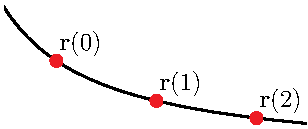
\includegraphics{parCurve.pdf}
\end{center}
\end{efig}
While in some applications $t$ will indeed be ``time'', it does not
have to be. It can be simply a parameter that is used to label the
different points on the curve that $\vr(t)$ sweeps out. We then say 
that $\vr(t)$ provides a parameterization of the curve.

\begin{eg}[Parametrization of  $x^2+y^2=a^2$]\label{eg:paramCircle}
While we will often use $t$ as the parameter in a parametrized curve $\vr(t)$,
there is no need to call it $t$. Sometimes it is natural to use a different 
name for the parameter. For example, consider the circle $x^2+y^2=a^2$.
It is natural to use the angle $\theta$ in the sketch below to label
the point $\big(a\cos\theta\,,\,a\sin\theta\big)$ on the circle. 
\begin{efig}
\begin{center}
     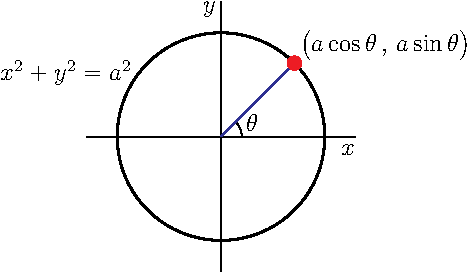
\includegraphics{parCircle.pdf}
\end{center}
\end{efig}
That is,
\begin{equation*}
\vr(\theta) = \big(a\cos\theta\,,\,a\sin\theta\big)\qquad
0\le \theta < 2\pi
\end{equation*}
is a parametrization of the circle $x^2+y^2=a^2$. Just looking at the figure above, it is clear that, as $\theta$ runs from $0$ to $2\pi$, $\vr(\theta)$
traces out the full circle. 

However beware that just knowing that 
$\vr(t)$ lies on a specified curve does not guarantee that, as $t$ varies,
$\vr(t)$ covers the entire curve. For example, as $t$ runs over the whole
real line, $\frac{2}{\pi}\arctan(t)$ runs over the interval $(-1,1)$.
For all $t$,
\begin{equation*}
\vr(t) = \big(x(t),y(t)\big) 
       = a\left(\frac{2}{\pi}\arctan(t)\,,\,
                \sqrt{1-\frac{4}{\pi^2}\arctan^2(t)}\,\right)
\end{equation*}
is well-defined and obeys $x(t)^2+y(t)^2=a^2$. But this $\vr(t)$ does not
cover the entire circle because $y(t)$ is always positive.

\end{eg}

\begin{eg}[Parametrization of  $(x-h)^2+(y-k)^2=a^2$]\label{eg:paramCircleB}
We can tweak the parametrization of Example \ref{eg:paramCircle} to get
a parametrization of the circle of radius $a$ that is centred on $(h,k)$.
One way to do so is to redraw the sketch of Example \ref{eg:paramCircle}
with the circle translated so that its centre is at $(h,k)$.
\begin{efig}
\begin{center}
     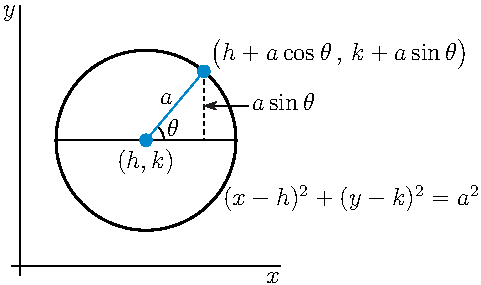
\includegraphics{parCirclehk.pdf}
\end{center}
\end{efig}
We see from the sketch that 
\begin{equation*}
\vr(\theta) = \big(h+a\cos\theta\,,\,k+a\sin\theta\big)\qquad
0\le \theta< 2\pi
\end{equation*}
is a parametrization of the circle $(x-h)^2+(y-k)^2=a^2$.

A second way to come up with this parametrization is to observe that 
we can turn the trig identity $\cos^2 t + \sin^2 t=1$ into 
the equation $(x-h)^2+(y-k)^2=a^2$ of the circle by
\begin{itemize}
\item
multiplying the trig identity by $a^2$ to get
$(a\cos t)^2 +(a\sin t)^2 =a^2$ and then
\item
setting $\ a\cos t=x-h\ $ and $\ a\sin t=y-k\ $, which turns  $(a\cos t)^2 +(a\sin t)^2 =a^2$ into $(x-h)^2+(y-k)^2=a^2$.
\end{itemize}
\end{eg}

\begin{eg}[Parametrization of  $\frac{x^2}{a^2}+\frac{y^2}{b^2}=1$ and of
$x^{2/3}+y^{2/3}=a^{2/3}$]    \label{eg:paramEllipse}

We can build parametrizations of the curves $\frac{x^2}{a^2}+\frac{y^2}{b^2}=1$ 
and $x^{2/3}+y^{2/3}=a^{2/3}$ from the trig identity $\cos^2 t + \sin^2 t=1$,
like we did in the second part of the last example.
\begin{itemize}
\item
Setting $\ \cos t=\frac{x}{a}\ $ and $\ \sin t=\frac{y}{b}\ $ turns  
$\cos^2 t +\sin^2 t =1$ into $\frac{x^2}{a^2}+\frac{y^2}{b^2}=1$.

\item
Setting $\ \cos t= \big(\frac{x}{a}\big)^{\frac{1}{3}}\ $ and 
$\ \sin t=\big(\frac{y}{a}\big)^{\frac{1}{3}}\ $ turns  
$\cos^2 t +\sin^2 t =1$ into $\frac{x^{2/3}}{a^{2/3}}+\frac{y^{2/3}}{a^{2/3}}=1$.
\end{itemize}
So
\begin{alignat*}{3}
\vr(t) &= \big(a\cos t\,,\,b\sin t\big)\qquad &0\le t< 2\pi
\\
\vr(t) &= \big(a\cos^3 t\,,\,a\sin^3 t\big) &0\le t< 2\pi
\end{alignat*}
give parametrizations of $\frac{x^2}{a^2}+\frac{y^2}{b^2}=1$ 
and $x^{2/3}+y^{2/3}=a^{2/3}$, respectively. To see that running $t$ from $0$ to $2\pi$ runs $\vr(t)$ once around the curve, look at the figures below.
\begin{wfig}
\begin{center}
     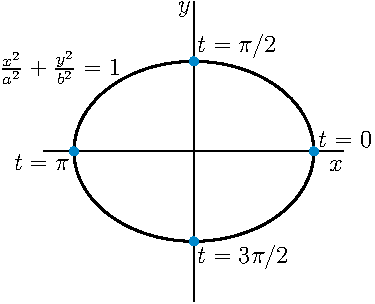
\includegraphics{parEllipse.pdf}\quad
     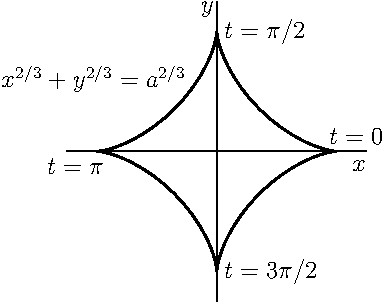
\includegraphics{astroid4.pdf}
\end{center}
\end{wfig}
The curve $x^{2/3}+y^{2/3}=a^{2/3}$ is called an astroid. From its equation,
we would expect its sketch to look like a deformed circle. But it is probably 
not so obvious that it would have the pointy bits of the right hand figure.
We will not explain here why they arise. The astroid is studied in some 
detail in Example \ref{eg:astroid}.
In particular, the above sketch is carefully developed there.  
 
\end{eg}

\begin{eg}[Parametrization of  $e^y=1+x^2$]\label{eg:paramMessy}
A very easy method that can often create parametrizations for a curve is to use $x$ or $y$ as a parameter. Because we can solve $e^y=1+x^2$ for $y$ as a function of $x$, namely $y=\ln\big(1+x^2\big)$, we can use $x$ as 
the parameter simply by setting $t=x$. This gives the parametrization
\begin{equation*}
\vr(t) = \big(t\,,\,\ln(1+t^2)\big)\qquad -\infty<t<\infty
\end{equation*}  
\end{eg}

\begin{eg}[Parametrization of  $x^2+y^2=a^2$, again]\label{eg:paramCircleC}
It is also quite common that one can use either $x$ or $y$ to parametrize part of, but all of, a curve. A simple example is the circle $x^2+y^2=a^2$.
For each $-a<x<a$, there are two points on the circle with that value of $x$.
So one cannot use $x$ to parametrize the whole circle.
Similarly, for each $-a<y<a$, there are two points on the circle with that value of $y$. So one cannot use $y$ to parametrize the whole circle. On the other 
hand
\begin{alignat*}{3}
\vr(t) &= \big(t\,,\,\sqrt{a^2-t^2}\big)\qquad &-a<t<a \\
\vr(t) &= \big(t\,,\,-\sqrt{a^2-t^2}\big)\qquad &-a<t<a
\end{alignat*}
provide parametrizations of the top half and bottom half, respectively,
of the circle using $x$ as the parameter, and
\begin{alignat*}{3}
\vr(t) &= \big(\sqrt{a^2-t^2}\,,\,t\big)\qquad &-a<t<a \\
\vr(t) &= \big(-\sqrt{a^2-t^2}\,,\,t\big)\qquad &-a<t<a
\end{alignat*}
provide parametrizations of the right half and left half, respectively,
of the circle using $y$ as the parameter.
\end{eg}

\begin{eg}[Unparametrization of  $\vr(t)=(\cos t, 7-t)$] \label{eg:unparam}
In this example, we will undo the parametrization $\vr(t)=(\cos t, 7-t)$
and find the Cartesian equation of the curve in question. We may rewrite the
parametrization as
\begin{align*}
x&=\cos t \\
y&=7-t
\end{align*}
Note that we can eliminate the parameter $t$ simply by using the second equation 
to solve for $t$ as a function of $y$. Namely $t=7-y$. Substituting this
into the first equation  gives us the Cartesian equation
\begin{equation*}
x=\cos(7-y)
\end{equation*}
\end{eg}

Curves often arise as the intersection of two surfaces. For example,
the intersection of the ellipsoid $x^2+\frac{y^2}{2}+\frac{z^2}{3}=1$
with the paraboloid $z=x^2+2y^2$ is the blue curve in the figure
below.
\vadjust{
\begin{nfig}
\begin{center}
    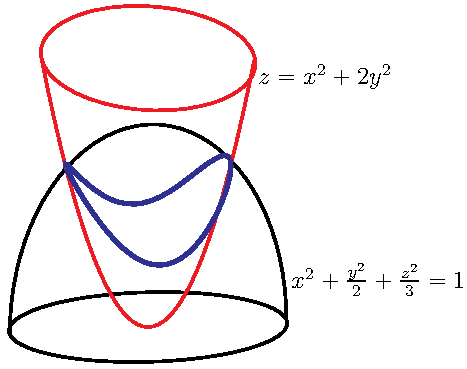
\includegraphics{stokes6.pdf}
\end{center}
\end{nfig}
}
One way to parametrize such curves is to
choose one of the three coordinates $x$, $y$, $z$ as the parameter,
and solve the two given equations for the remaining two coordinates,
as functions of the parameter. Here are two examples.

\begin{eg}\label{eg:paramIntersect}
The set of all $(x,y,z)$ obeying
\begin{alignat*}{3}
 x^3&-e^{3y}           &&=0 \\
 x^2&-e^{y} +z &&=0
\end{alignat*}
is a curve. We can choose to use $y$ as the parameter and think of 
\begin{alignat*}{3}
 x^3&    &&=e^{3y} \\
 x^2&+z  &&=e^{y}
\end{alignat*}
as a system of two equations for the two unknowns $x$ and $z$,
with $y$ being treated as a given constant, rather than as an unknown.
We can now solve the first equation for $x$, substitute the result into
the second equation, and finally solve for $z$.
\begin{alignat*}{7}
 x^3&    &&=e^{3y}  &&\implies x=e^y \\
 x^2&+z  &&=e^{y}   && &&\implies e^{2y}+z=e^y \implies z=e^y-e^{2y}
\end{alignat*}
So
\begin{equation*}
\vr(y) = \big(e^y\,,\,y\,,\,e^y-e^{2y}\big)
\end{equation*}
is a parametrization for the given curve.
\end{eg}


\begin{eg}\label{eg:paramIntersectB}
The previous example was rigged so that it was easy to solve
for $x$ and $z$ as functions of $y$. In practice it is not always
easy, or even possible, to do so. A more realistic example is 
the set of all $(x,y,z)$ obeying
\begin{alignat*}{3}
 x^2+\frac{y^2}{2}+\frac{z^2}{3}&=1  \\
 x^2+2y^2&=z
\end{alignat*}
which is the blue curve in the figure above. 
Substituting $x^2=z-2y^2$ (from the second equation)
into the first equation gives 
\begin{equation*}
-\frac{3}{2}y^2+z+\frac{z^2}{3}=1
\end{equation*}
or, completing the square,
\begin{equation*}
-\frac{3}{2}y^2 + \frac{1}{3}\Big(z+\frac{3}{2}\Big)^2 = \frac{7}{4}
\end{equation*}
If, for example, we are interested in points $(x,y,z)$ on the curve with 
$y\ge 0$, this can be solved to give $y$ as a function of $z$.
\begin{equation*}
y=\sqrt{\frac{2}{9}\Big(z+\frac{3}{2}\Big)^2-\frac{14}{12}}
\end{equation*}
Then $x^2=z-2y^2$ also gives $x$ as a function of $z$. If $x\ge 0$,
\begin{align*}
x&=\sqrt{z-\frac{4}{9}\Big(z+\frac{3}{2}\Big)^2+\frac{14}{6}} \\
&=\sqrt{\frac{4}{3}-\frac{4}{9}z^2-\frac{1}{3}z} 
\end{align*}
The other signs of $x$ and $y$ can be gotten by using the appropriate
square roots. In this example, $(x,y,z)$ is on the curve, i.e. satisfies
the two original equations, if and only if all of $(\pm x,\pm y, z)$ are also
on the curve.

\end{eg}


\section{Derivatives, Velocity, Etc.}\label{sec curve derivs}

This being a Calculus text, one of our main operations is differentiation.
We are now interested in parametrizations $\vr(t)$.
It is very easy and natural to extend our definition of derivative to $\vr(t)$
as follows.

\begin{defn}\label{def: curve deriv}
The derivative of the vector valued function $\vr(t)$ is defined to be
\begin{equation*}
\vr'(t) =  \diff{\vr}{t}(t)=\lim_{h\rightarrow 0}\frac{\vr(t+h)-\vr(t)}{h}
\qquad
\raisebox{-25pt}[25pt][20pt]{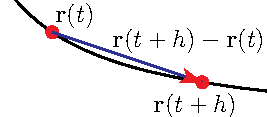
\includegraphics{parCurveDerivA.pdf}}
\end{equation*}
when the limit exists. In particular, if 
$\vr(t)=\big(x(t)\,,\,y(t)\,,\,z(t)\big)$, then
\begin{equation*}
\vr'(t)=\big(x'(t)\,,\,y'(t)\,,\,z'(t)\big)
\end{equation*}
That is, to differentiate a vector valued function of $t$, just differentiate
each of its components.
\end{defn}

And of course differentiation interacts with arithmetic operations, 
like addition, in the obvious way. Only a little more thought is required to 
see that differentiation interacts quite nicely with dot and cross 
products too.  Here are some examples.

\begin{eg}\label{eg:diffDot}
Let
\begin{align*}
\va(t)&= t^2\,\hi + t^4\,\hj + t^6\,\hk
\\
\vb(t)&= e^{-t}\,\hi + e^{-3t}\,\hj + e^{-5t}\,\hk
\\
\ga(t)&= t^2
\\
s(t)&= \sin t
\end{align*}
We are about to compute some derivatives. To make it easier to follow what is going on, we'll use some colour. When we apply the product rule
\begin{align*}
\diff{}{t}\big[f(t)\,g(t)\big]
&=\textcolor{blue}{f'(t)}\,g(t) + f(t)\,\textcolor{blue}{g'(t)}
\end{align*} 
we'll use blue to highlight the factors $f'(t)$ and $g'(t)$.
Here we go.
\begin{align*}
\ga(t)\,\vb(t) & = t^2e^{-t}\,\hi + t^2 e^{-3t}\,\hj + t^2 e^{-5t}\,\hk
\\
\implies \diff{}{t}\big[\ga(t)\vb(t)\big]
&=\big[\textcolor{blue}{2t} e^{-t}
           \textcolor{blue}{-}t^2\textcolor{blue}{e^{-t}}\big]\hi
  +\big[\textcolor{blue}{2t} e^{-3t}
           \textcolor{blue}{-3}t^2\textcolor{blue}{e^{-3t}}\big]\hj
  +\big[\textcolor{blue}{2t} e^{-5t}
          \textcolor{blue}{-5}t^2e^{-5t}\big]\hk
\\
&=\textcolor{blue}{2t}\big\{e^{-t}\,\hi + e^{-3t}\,\hj + e^{-5t}\,\hk\big\}
+ t^2
    \textcolor{blue}{\big\{-e^{-t}\,\hi -3 e^{-3t}\,\hj -5 e^{-5t}\,\hk\big\}}
\\
&=\textcolor{blue}{\ga'(t)}\vb(t)
         +\ga(t)\textcolor{blue}{\vb'(t)}
\end{align*}
and 
\begin{align*}
\va(t)\cdot\vb(t) & = t^2e^{-t} + t^4 e^{-3t} + t^6 e^{-5t}
\\
\implies \diff{}{t}\big[\va(t)\cdot\vb(t)\big]
&=\big[\textcolor{blue}{2t} e^{-t}
            \textcolor{blue}{-}t^2\textcolor{blue}{e^{-t}}\big]
  +\big[\textcolor{blue}{4t^3} e^{-3t}
            \textcolor{blue}{-3}t^4\textcolor{blue}{e^{-3t}}\big]
  +\big[\textcolor{blue}{6t^5} e^{-5t}
             \textcolor{blue}{-5}t^6\textcolor{blue}{e^{-5t}}\big]
\\
&=\big[\textcolor{blue}{2t} e^{-t}
            +\textcolor{blue}{4t^3} e^{-3t}
            +\textcolor{blue}{6t^5} e^{-5t}\big]
  +\big[\textcolor{blue}{-}t^2\textcolor{blue}{e^{-t}}
             \textcolor{blue}{-3}t^4\textcolor{blue}{e^{-3t}}
             \textcolor{blue}{-5t}^6\textcolor{blue}{e^{-5t}}\big]
\\
&=\textcolor{blue}{\big\{2t\,\hi+4t^3\,\hj+6t^5\,\hk\big\}}\cdot
           \big\{e^{-t}\,\hi + e^{-3t}\,\hj + e^{-5t}\,\hk\big\}\\&\hskip0.5in
  +\big\{t^2\,\hi + t^4\,\hj + t^6\,\hk\big\}\cdot
         \textcolor{blue}{\big\{-e^{-t}\,\hi-3e^{-3t}\,\hj-5e^{-5t}\,\hk\big\}}
\\
&=\textcolor{blue}{\va'(t)}\cdot\vb(t)+\va(t)\cdot\textcolor{blue}{\vb'(t)}
\end{align*}
and
\begin{align*}
\va(t)\times\vb(t) 
&=\det\left[\begin{matrix}\hi& \hj &\hk\\ 
                            t^2 & t^4 & t^6\\ 
                            e^{-t} & e^{-3t} & e^{-5t}\end{matrix}\right] \\
&=\hi\big(t^4 e^{-5t}-t^6 e^{-3t}) 
  -\hj(t^2 e^{-5t}- t^6 e^{-t}) 
   +\hk(t^2 e^{-3t}-t^4 e^{-t})
\\
\implies \diff{}{t}\big[\va(t)\times\vb(t)\big]
&=\ \hi\big(\ \textcolor{blue}{4t^3} e^{-5t}\ \ 
        -\ \textcolor{blue}{6t^5} e^{-3t}) 
  \ -\ \hj(\ \textcolor{blue}{2t} e^{-5t}
      \ -\  \textcolor{blue}{6t^5} e^{-t}) 
   +\hk(\ \textcolor{blue}{2t} e^{-3t}
   \ -\ \textcolor{blue}{4t^3} e^{-t}) \\&\hskip0.1in
 +\hi\big(\textcolor{blue}{-5}t^4 \textcolor{blue}{e^{-5t}}
           \textcolor{blue}{+3}t^6 \textcolor{blue}{e^{-3t}}) 
  -\hj(\textcolor{blue}{-5}t^2 \textcolor{blue}{e^{-5t}}
          \textcolor{blue}{+} t^6 \textcolor{blue}{e^{-t}}) 
   +\hk(\textcolor{blue}{-3}t^2 \textcolor{blue}{e^{-3t}}
     \textcolor{blue}{+}t^4 \textcolor{blue}{e^{-t}})
\\
&=\textcolor{blue}{\big\{2t\,\hi+4t^3\,\hj+6t^5\,\hk\big\}}\times
           \big\{e^{-t}\,\hi + e^{-3t}\,\hj + e^{-5t}\,\hk\big\}\\&\hskip0.1in
  +\big\{t^2\,\hi + t^4\,\hj + t^6\,\hk\big\}\times
         \textcolor{blue}{\big\{-e^{-t}\,\hi-3e^{-3t}\,\hj-5e^{-5t}\,\hk\big\}}
\\
&=\textcolor{blue}{\va'(t)}\times\vb(t)+\va(t)\times\textcolor{blue}{\vb'(t)}
\end{align*}
and
\begin{align*}
\va\big(s(t)\big)
&=(\sin t)^2\,\hi +(\sin t)^4\,\hj + (\sin t)^6\,\hk
\\
\implies \diff{}{t}\big[\va\big(s(t)\big)\big]
&=2(\sin t)\cos t\,\hi +4(\sin t)^3\cos t\,\hj + 6(\sin t)^5\cos t\,\hk
\\
&=\big\{2(\sin t)\,\hi +4(\sin t)^3\hj + 6(\sin t)^5\hk\big\}\cos t 
\\
&=\va'\big(s(t)\big)\,s'(t)
\end{align*}
\end{eg}

Of course these examples extend to general (differentiable)
$\va(t)$, $\vb(t)$, $\ga(t)$ and $s(t)$ and give us (most of) the following theorem. 

\begin{theorem}[Arithmetic of differentiation]\label{thm:DIFFalgebra}
Let 
\begin{itemize}\itemsep1pt \parskip0pt \parsep0pt %\itemindent-15pt
\item[$\circ$]
$\va(t),\vb(t)$ be vector valued differentiable functions of $t\in\bbbr$
that take values in $\bbbr^n$ and
\item[$\circ$]
 $\alpha,\beta \in \mathbb{R}$ be constants and 
\item[$\circ$]
 $\ga(t)$ and $s(t)$ be real valued differentiable functions of $t\in\bbbr$
\end{itemize}
Then
\begin{alignat*}{5}
&\text{(a)}\quad &&\diff{}{t}\big[\alpha\,\va(t)+\beta\,\vb(t)\big]
         =\alpha\,\va'(t)+\beta\,\vb'(t)
           &&\text{(linear combination)}
\\
&\text{(b)} &&\diff{}{t}\big[\ga(t)\vb(t)\big]
         =\ga'(t)\vb(t)+\ga(t)\vb'(t)
           &&\text{(multiplication by scalar function)}
\\
&\text{(c)} &&\diff{}{t}\big[\va(t)\cdot\vb(t)\big]
         =\va'(t)\cdot\vb(t)+\va(t)\cdot\vb'(t)
           &&\text{(dot product)}
\\
&\text{(d)} &&\diff{}{t}\big[\va(t)\times\vb(t)\big]
         =\va'(t)\times\vb(t)+\va(t)\times\vb'(t)
           \ \ &&\text{(cross product)}
\\
&\text{(e)} &&\diff{}{t}\big[\va\big(s(t)\big)\big]
         =\va'\big(s(t)\big)\,s'(t)
           &&\text{(composition)}
\end{alignat*}
%\begin{enumerate}[(a)]
%\item $\diff{}{t}\big[\alpha\,\va(t)+\beta\,\vb(t)\big]
%         =\alpha\,\va'(t)+\beta\,\vb'(t)$
%%\item $\diff{}{t}\big[\al\vb(t)\big]
%%         =\al\vb'(t)$
%\item $\diff{}{t}\big[\ga(t)\vb(t)\big]
%         =\ga'(t)\vb(t)+\ga(t)\vb'(t)$
%\item $\diff{}{t}\big[\va(t)\cdot\vb(t)\big]
%         =\va'(t)\cdot\vb(t)+\va(t)\cdot\vb'(t)$
%\item $\diff{}{t}\big[\va(t)\times\vb(t)\big]
%         =\va'(t)\times\vb(t)+\va(t)\times\vb'(t)$
%\item $\diff{}{t}\big[\va\big(s(t)\big)\big]
%         =\va'\big(s(t)\big)\,s'(t)$
%\end{enumerate}
\end{theorem}

Let's think about the geometric significance of $\vr'(t)$.
In particular, let's think about the relationship between $\vr'(t)$
and distances along the curve.
The derivative $\vr'(t)$ is the limit of   $\frac{\vr(t+h)-\vr(t)}{h}$ as $h\rightarrow 0$. 
The numerator, $\vr(t+h)-\vr(t)$, is the vector with head at $\vr(t+h)$ 
and tail at $\vr(t)$. 
\begin{efig}
\begin{center}
     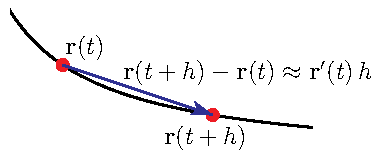
\includegraphics{parCurveDeriv.pdf}
\end{center}
\end{efig}
When $h$ is very small this vector
\begin{itemize}\itemsep1pt \parskip0pt \parsep0pt %\itemindent-15pt
\item[$\circ$]
has the essentially the same direction as the tangent vector to the curve at $\vr(t)$ and
\item[$\circ$]
has length being essentially the length of the part of the curve between
$\vr(t)$ and $\vr(t+h)$.
\end{itemize}
Taking the limit as $h\rightarrow 0$ yields that
\begin{itemize}\itemsep1pt \parskip0pt \parsep0pt %\itemindent-15pt
\item[$\circ$]
$\vr'(t)$ is a tangent vector to the curve at $\vr(t)$ that points in
the direction of increasing $t$ and
\item[$\circ$]
if $s(t)$ is the length of the part of the curve between
$\vr(0)$ and $\vr(t)$, then  $\diff{s}{t}(t)=\big|\diff{\vr}{t}(t)\big|$.
\end{itemize}
This is worth stating formally.

%%%%%%%%%%%%%%%
\begin{lemma}\label{lem:CVtanArclen}
Let $\vr(t)$ be a parametrized curve.
\begin{enumerate}[(a)]
\item 
Denote by $\hat\vT(t)$ the unit tangent vector to the curve 
at $\vr(t)$ pointing in the direction of increasing $t$. If
$\vr'(t)\ne 0$
then
\begin{equation*}
\hat\vT(t) = \frac{\vr'(t)}{|\vr'(t)|}
\end{equation*}

\item
Denote by $s(t)$ the length of the part of the curve between
$\vr(0)$ and $\vr(t)$. Then
\begin{align*}
\diff{s}{t}(t)&=\Big|\diff{\vr}{t}(t)\Big| \\
s(T)-s(T_0)&= \int_{T_0}^T \left|\diff{\vr}{t}(t)\right|\,\dee{t}\qquad
\raisebox{-20pt}{\smash{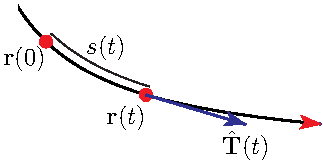
\includegraphics{parCurveDerivB.pdf}}}
\end{align*}

\item
In particular, if the parameter happens to be arc length, i.e. if $t=s$,
so that $\diff{s}{s}=1$, then
\begin{equation*}
\left|\diff{\vr}{s}(s)\right|=1\qquad
\hat\vT(s) = \vr'(s)
\end{equation*}


\end{enumerate}
\end{lemma}

As an application, we have the

\begin{lemma}\label{lem:CVvelocityEtc}
If $\vr(t)=\big(x(t)\,,\,y(t)\,,\,z(t)\big)$ is the position of a 
particle at time $t$, then
\begin{align*}
\text{position at time $t$}
       &=\vr(t)=\big(x(t)\,,\,y(t)\,,\,z(t)\big) \\
\text{velocity at time $t$}
       &=\vv(t)=\vr'(t)=\big(x'(t)\,,\,y'(t)\,,\,z'(t)\big) 
        = \diff{s}{t}(t)\,\hat\vT(t)\\
\text{speed at time $t$}
       &= \diff{s}{t}(t)=|\vv(t)|=|\vr'(t)|=\sqrt{(x'(t)^2+y'(t)^2+z'(t)^2} \\
\text{acceleration at time $t$}
       &=\va(t)=\vr''(t)=\vv'(t)=\big(x''(t)\,,\,y''(t)\,,\,z''(t)\big) \\
\intertext{and the distance travelled between times $T_0$ and $T$ is}
  s(T)-s(T_0)&= \int_{T_0}^T \Big|\diff{\vr}{t}(t)\Big|\,\dee{t}
       = \int_{T_0}^T \sqrt{(x'(t)^2+y'(t)^2+z'(t)^2}\,\dee{t}
\end{align*}
\end{lemma}
Note that the velocity $\vv(t) = \vr'(t)$ is a vector quantity while the
speed $\diff{s}{t}(t)=|\vr'(t)|$ is a scalar quantity.


\begin{eg}[Circumference of a circle]\label{eg:paramCircleTan}
In general it can be quite difficult to compute arc lengths.
So, as an easy warmup example, we will compute the circumference of the circle
$x^2+y^2=a^2$. We'll also find a unit tangent to the circle at any point on
the circle. We'll use the parametrization
\begin{equation*}
\vr(\theta) = \big(a\cos\theta\,,\,a\sin\theta\big)\qquad
0\le \theta\le 2\pi
\end{equation*}
of Example \ref{eg:paramCircle}. Using Lemma \ref{lem:CVtanArclen},
but with the parameter $t$ renamed to $\theta$
\begin{align*}
\vr'(\theta) &= a\big(-\sin\theta\,,\cos\theta\big) \\
\hat\vT(\theta) &= \frac{\vr'(\theta)}{|\vr'(\theta)|}
               =  \big(-\sin\theta\,,\cos\theta\big) \\
\diff{s}{\theta}(\theta)&=\big|\vr'(\theta)\big| = a\\
s(\Theta)-s(0)&= \int_{0}^\Theta \big|\vr'(\theta)\big|\,\dee{\theta}
          =a\Theta
\end{align*}
As\footnote{You might guess that $\Theta$ is a capital Greek theta. You'd be right.} $s(\Theta)$ is the arc length of the part of the circle with 
$0\le\theta\le\Theta$, the circumference of the whole circle is
\begin{equation*}
s(2\pi) = 2\pi a
\end{equation*} 
which is reassuring, since this formula has been known\footnote{The earliest known written approximations of $\pi$, in Egypt and Babylon, date 
from 1900--1600BC. The first recorded algorithm for rigorously evaluating $\pi$
was developed by Archimedes around 250 BC. The first use of the symbol $\pi$,
for the ratio between the circumference of a circle and its diameter,
in print was in 1706 by William Jones.}
for thousands of years.%
\vadjust{
\begin{efig}
\begin{center}
     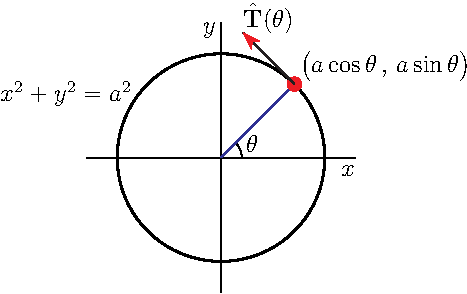
\includegraphics{parCircleT.pdf}
\end{center}
\end{efig}
}
The formula $s(\Theta)-s(0)=a\Theta$ also makes sense --- the part of the 
circle with $0\le\theta\le\Theta$ is the fraction $\frac{\Theta}{2\pi}$
of the whole circle, and so should have length $\frac{\Theta}{2\pi}\times
2\pi a$. Also note that
\begin{equation*}
\vr(\theta)\cdot\hat\vT(\theta) = \big(a\cos\theta\,,\,a\sin\theta\big)
\cdot \big(-\sin\theta\,,\cos\theta\big)
=0
\end{equation*}
so that the tangent to the circle at any point is perpendicular
to the radius vector of the circle at that point. This is another geometric fact 
that has been known\footnote{It is Proposition 18 in Book 3 of Euclid's Elements. It was published around 300BC.} for thousands of years.
\end{eg}


\begin{eg}[Arc length of a helix]\label{eg:paramHelix}
Consider the curve
\begin{equation*}
\vr(t) = 6\sin(2t)\hi + 6\cos(2t)\hj +5t\hk
\end{equation*}
where the standard basis vectors $\hi = (1,0,0)$, $\hj=(0,1,0)$ 
and $\hk =(0,0,1)$.
We'll first sketch it, by observing that
\begin{itemize}\itemsep1pt \parskip0pt \parsep0pt %\itemindent-15pt
\item[$\circ$] $x(t)=6\sin(2t)$ and $y(t) =6\cos(2t)$ obey
$x(t)^2+y(t)^2 = 36 \sin^2(2t) + 36\cos^2(2t) = 36$. So all points of the
curve lie on the cylinder $x^2+y^2=36$ and
\item[$\circ$] as $t$ increases, $\big(x(t),y(t)\big)$ runs clockwise 
around the circle $x^2+y^2=36$ and at the same time $z(t) = 5t$ 
just increases linearly.
\end{itemize}
Our curve is the helix
\begin{efig}
\begin{center}
     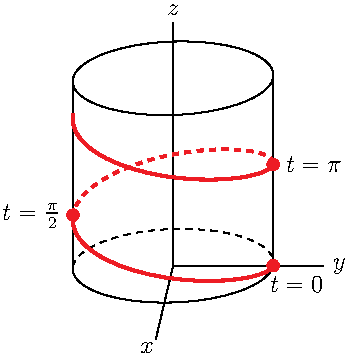
\includegraphics{helix4.pdf}
\end{center}
\end{efig}
We have marked three points of the curve on the above sketch. The first has
$t=0$ and is $0\hi+6\hj+0\hk$. The second has $t=\frac{\pi}{2}$ and is $0\hi-6\hj+\frac{5\pi}{2}\hk$, and the third has $t=\pi$ and is 
$0\hi+6\hj+5\pi\hk$.
We'll now use Lemma \ref{lem:CVtanArclen} to find a unit tangent
$\hat\vT(t)$ to the curve at $\vr(t)$ and also the arclength of the part of curve between $t=0$ and $t=\pi$.
\begin{align*}
\vr(t) &= 6\sin(2t)\hi + 6\cos(2t)\hj +5t\hk \\
\vr'(t) &= 12\cos(2t)\hi -12\sin(2t)\hj +5\hk \\
\diff{s}{t}(t)&=\big|\vr'(t)\big| 
=\sqrt{12^2\cos^2(2t) +12^2\sin^2(2t)+5^2}
= \sqrt{12^2+5^2} \\
&= 13\\
\hat\vT(t) &= \frac{\vr'(t)}{|\vr'(t))|}
               =  \frac{12}{13}\cos(2t)\hi -\frac{12}{13}\sin(2t)\hj +\frac{5}{13}\hk \\
s(\pi)-s(0)&= \int_{0}^\pi \big|\vr'(t)\big|\,\dee{t}
          =13\pi
\end{align*}
\end{eg}
\goodbreak

\begin{eg}[Velocity and acceleration]\label{eg:velAccel}
Imagine that, at time $t$, a particle is at 
\begin{equation*}
\vr(t) = \left[h+a\cos\left(2\pi\frac{t}{T}\right)\right]\hi
            +\left[k+a\sin\left(2\pi\frac{t}{T}\right)\right]\hj
\end{equation*}
As $|\vr(t) -h\,\hi-k\,\hj| = a$, the particle is running around the circle of radius $a$ centred on $(h,k)$. When $t$ increases by $T$, the argument, $2\pi\frac{t}{T}$, of $\cos\left(2\pi\tfrac{t}{T}\right)$ and 
$\sin\left(2\pi\tfrac{t}{T}\right)$ increases by exactly $2\pi$ and the particle runs exactly once around the circle. In particular, it travels a distance 
$2\pi a$. So it is moving at speed  $\frac{2\pi a}{T}$. 
According to Lemma \ref{lem:CVvelocityEtc}, it has 
\begin{align*}
\text{velocity }
       &=\vr'(t)=-\frac{2\pi a}{T}\sin\left(2\pi\frac{t}{T}\right)\hi
            +\frac{2\pi a}{T}\cos\left(2\pi\frac{t}{T}\right)\hj
      \\
\text{speed}
       &= \diff{s}{t}(t)=|\vr'(t)|=\frac{2\pi a}{T} \\
\text{acceleration}
       &=\vr''(t)
        =-\frac{4\pi^2 a}{T^2}\cos\left(2\pi\frac{t}{T}\right)\hi
            -\frac{4\pi^2 a}{T^2}\sin\left(2\pi\frac{t}{T}\right)\hj 
        = - \frac{4\pi^2}{T^2}\big[\vr(t) -h\,\hi-k\,\hj\big]
\end{align*}
Here are some observations.
\begin{itemize}
\item 
The velocity $\vr'(t)$ has dot product zero with $\vr(t) -h\,\hi-k\,\hj$, which is the radius vector from the centre of the circle to the particle.
So the velocity is perpendicular to the radius vector, and hence parallel to the 
tangent vector of the circle at $\vr(t)$.
\item 
The speed given by Lemma \ref{lem:CVvelocityEtc} is exactly the speed
we found above, just before we started applying Lemma \ref{lem:CVvelocityEtc}.
\item 
The acceleration $\vr''(t)$ points in the direction opposite to the radius 
vector.
\end{itemize}

\begin{efig}
\begin{center}
     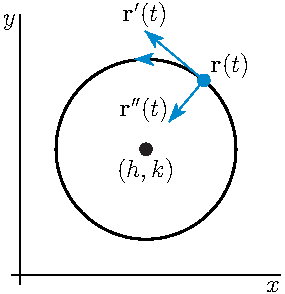
\includegraphics{circleVA.pdf}
\end{center}
\end{efig}
\end{eg}

\begin{eg}[Perimeter of the astroid]\label{eg:astroid}
In this example, we find the perimeter of the astroid\footnote{
Astroid should not be confused with asteroid, though both words derive 
from the Greek word for star.}
\begin{equation*}
x^{2/3}+y^{2/3} = a^{2/3}
\end{equation*}
A geometric construction of this curve, as well as a derivation of its equation is given in the optional section \ref{sec:astroid} later.  We'll start by finding a convenient
parametrization. 
\begin{itemize}\itemsep1pt \parskip0pt \parsep0pt %\itemindent-15pt
\item[$\circ$]
To do so, notice that $x^{2/3}+y^{2/3} = a^{2/3}$ looks somewhat like the
equation of the circle $x^2+y^2=a^2$. 
\item[$\circ$]
The standard parametrization of the circle, namely
$x=a\cos t$, $y=a \sin t$ works because of the elementary trig identity $\cos^2t+\sin^2t=1$.
\item[$\circ$]
If we can arrange that $x(t)^{2/3} = a^{2/3}\cos^2 t$ and $y(t)^{2/3}=a^{2/3}\sin^2 t$, then the same elementary trig identity will give $x(t)^{2/3}+y(t)^{2/3} = a^{2/3}$, as desired. 
\item[$\circ$]
But 
of course its easy to arrange that: just solve  $x(t)^{2/3} = a^{2/3}\cos^2 t$ for $x(t)$, 
namely $x(t) = a\cos^3t$, and solve $y(t)^{2/3}=a^{2/3}\sin^2 t$ for $y(t)$,
namely $y(t)=a\sin^3 t$. 
\end{itemize}
Our parametrization is 
\begin{equation*}
\vr(t) = a\cos^3t\,\hi + a\sin^3 t\,\hj
\end{equation*}
By Lemma \ref{lem:CVtanArclen}
\begin{align*}
\vr(t) &= a\cos^3t\,\hi + a\sin^3 t\,\hj \\
\vr'(t) &= -3a\sin t\cos^2t\,\hi + 3a\sin^2 t\cos t\,\hj \\
\diff{s}{t}(t)&=\big|\vr'(t)\big| 
= \sqrt{9a^2\sin^2t\cos^4t + 9a^2\sin^4t\cos^2t} \\
& = 3a \sqrt{\sin^2t\cos^2t(\cos^2t+\sin^2t)} \\
 &=3a\big|\sin t\cos t\big| \\
\hat\vT(t) &= \frac{\vr'(t)}{|\vr'(t))|}
=  \frac{\sin t\cos t}{|\sin t\cos t|}\ \big(-\cos t\,\hi+\sin t\,\hj\big)
\\
 &=  \sgn\!\big(\!\sin t\cos t\big)\ \big(-\cos t\,\hi+\sin t\,\hj\big) 
\end{align*}
Here $\sgn\!\big(\!\sin t\cos t\big)$ means ``the sign of $\sin t\cos t$'', i.e $+1$ when $\sin t\cos t>0$ and $-1$ when $\sin t\cos t<0$. So
\begin{align*}
\hat\vT(t) 
 &=\left.\begin{cases}1&\text{if $\ \sin t>0,\ \cos t>0\ \ $ 
                              or $\ \ \sin t<0,\ \cos t<0$}\\
                           -1&\text{if $\ \sin t>0,\ \cos t<0\ \ $ 
                              or $\ \ \sin t<0,\ \cos t>0$}
                \end{cases}\right\}\big(-\cos t\,\hi+\sin t\,\hj\big)
\\
 &=\left.\begin{cases}1&\text{if $\ \ 0< t<\frac{\pi}{2}\ \ $ 
                                            or $\ \ \pi< t<\frac{3\pi}{2}$}\\
                           -1&\text{if $\ \ \frac{\pi}{2}<t<\pi\ \ $ 
                                          or $\ \ \frac{3\pi}{2}<t<2\pi$}
                \end{cases}\right\}\big(-\cos t\,\hi+\sin t\,\hj\big)
\end{align*}

Before we go on to sketch the astroid and compute its perimeter, we can 
make a few observations that will simplify our lives. 
\begin{itemize}\itemsep1pt \parskip0pt \parsep0pt %\itemindent-15pt
\item[$\circ$]
The signs of both components
of $\vr(t)$ are the same as the signs of the components of
$\cos t\,\hi +\sin t\,\hj$; and the signs of both components
of $\vr'(t)$ are the same as the signs of the components of
$-\sin t\,\hi +\cos t\,\hj$.
Consequently the astroid looks somewhat like a circle in that
\begin{itemize}\itemsep1pt \parskip0pt \parsep0pt %\itemindent-15pt
\item 
when $0\le t\le \frac{\pi}{2}$, $\vr(t)$ lies in the first quadrant
and moves upward and to the left as $t$ increases and
\item 
when $\frac{\pi}{2}\le t\le \pi$, $\vr(t)$ lies in the second 
quadrant and moves downward and to the left as $t$ increases and
\item 
when $\pi\le t\le \frac{3\pi}{2}$, $\vr(t)$ lies in the third quadrant
and moves downward and to the right as $t$ increases and
\item 
when $\frac{3\pi}{2}\le t\le 2\pi$, $\vr(t)$ lies in the fourth
quadrant and moves upward and to the right as $t$ increases and
\item 
$\vr(2\pi)=\vr(0)$ so that the astroid is a closed curve that
circumnavigates the origin exactly once as $t$ runs from $0$ to $2\pi$.
\end{itemize}

\item[$\circ$]
Something weird happens at those values of $t$ where $\sin t\cos t$ changes sign\footnote{Like a cross-walk sign.},
i.e. at $t=0$, $\frac{\pi}{2}$, $\pi$, $\frac{3\pi}{2}$, etc. Namely $\hat T(t)$ 
flips. To be precise
\begin{align*}
\lim_{t\rightarrow 0-}\hat T(t) 
&=\lim_{t\rightarrow 0-}  \sgn\!\big(\!\sin t\cos t\big)\   
         \lim_{t\rightarrow 0-}\big(-\cos t\,\hi+\sin t\,\hj\big)
= \hi \\
\lim_{t\rightarrow 0+}\hat T(t) 
&= \lim_{t\rightarrow 0+}\sgn\!\big(\!\sin t\cos t\big)\ 
\lim_{t\rightarrow 0+}\big(-\cos t\,\hi+\sin t\,\hj\big)
=-\hi \\
\end{align*}
and 
\begin{align*}
\lim_{t\rightarrow \pi/2-}\hat T(t) 
&= \lim_{t\rightarrow \pi/2-}\sgn\!\big(\!\sin t\cos t\big)\ 
\lim_{t\rightarrow \pi/2-}\big(-\cos t\,\hi+\sin t\,\hj\big)
=\hj \\
\lim_{t\rightarrow \pi/2+}\hat T(t) 
&= \lim_{t\rightarrow \pi/2+}\sgn\!\big(\!\sin t\cos t\big)\ 
\lim_{t\rightarrow \pi/2+}\big(-\cos t\,\hi+\sin t\,\hj\big)
=-\hj 
\end{align*}
and so on. This signals cusps in the curve at $t=0$, i.e. at $\vr(0) = a\hi$,
and at $t=\frac{\pi}{2}$, i.e. at $\vr(\frac{\pi}{2}) = a\hj$, and so on. So
while the astroid looks somewhat like a circle, it has cusps at $\pm a\hi$ and $\pm a\hj$. Here is the sketch.
\begin{efig}
\begin{center}
     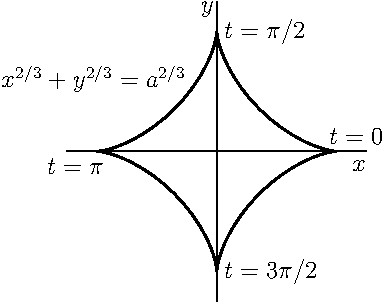
\includegraphics{astroid4.pdf}
\end{center}
\end{efig}
\item[$\circ$] The astroid is invariant under reflections in the $x$-axis and in the 
$y$-axis. That is, $x^{2/3}+y^{2/3} = a^{2/3}$ is invariant under $x\rightarrow -x$ 
and also under $y\rightarrow -y$. So to find the whole perimeter, it suffices to find the 
arc length of the part of the astroid in the first quadrant, and then multiply by $4$.
\begin{align*}
\text{perimeter}
&=4\int_0^{\pi/2}\diff{s}{t}\ \dee{t}
 = 4\int_0^{\pi/2}3a\sin t\cos t\ \dee{t}
 = 6a\int_0^{\pi/2}\sin(2t)\ \dee{t} \\
 &=6a\Big[-\frac{\cos(2t)}{2}\Big]_0^{\pi/2}
=6a
\end{align*}
\end{itemize}

\end{eg}


\begin{eg}[$\vr'(t)=\vZero$]\label{eg:zeroSpeed}
In the last example, we found that the astroid  had
cusps at those points $\vr(t)$ where the velocity $\vr'(t)$ vanished.
In this example, we will explore a little further what can happen when
$\vr'(t)=\vZero$. 

Suppose that you are out for a walk and that your position
at time $t$ is $\vr(t)$. If at some time you have nonzero velocity,
it is very hard for you to  change your direction of motion 
discontinuously\footnote{For your velocity to jump
discontinuously, your acceleration has to be infinite, which requires an 
infinite force. You might not look so healthy afterwards}. On the other hand, when 
$\vr'(t)=0$, you are not moving at all and it is easy for you to turn and
leave in any direction you choose. You could reverse direction completely,
or make a sharp left turn, or not change direction at all. Here are examples 
of all of these. They all have $\vr'(t)=0$. They are sketched below.
\begin{alignat*}{3}
\vr_1(t) &= (t^5, t^2) &
\vr_1'(t)&= (5t^4, 2t) 
\\[0.1in]
\vr_2(t) &= \left.\begin{cases} (t^2, 0) & \text{if $t\ge 0$} \\
                        (0 , t^2) & \text{if $t\le 0$}
          \end{cases}\right\}\qquad &
\vr_2'(t)&= \left.\begin{cases} (2t, 0) & \text{if $t\ge 0$} \\
                        (0 , 2t) & \text{if $t\le 0$}
          \end{cases} \right\}
\\[0.1in]
\vr_3(t) &= (t^3, 0) &
\vr_3'(t) &= (3t^2, 0) 
\end{alignat*}
\begin{efig}
\begin{center}
     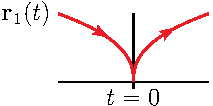
\includegraphics{cuspA.pdf}\qquad\qquad
     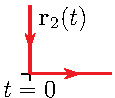
\includegraphics{cuspB.pdf}\qquad\qquad
     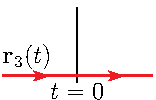
\includegraphics{nocusp.pdf}
\end{center}
\end{efig}


\end{eg}

\begin{eg}[Corkscrew]\label{eg:corkscrew}
We'll find the arc length of 
\begin{equation*}
\vr(t) = t\cos t\,\hi + t\sin t\,\hj +t\,\hk\qquad
0\le t\le\sqrt{2}
\end{equation*}
We'll first sketch it, by observing that
\begin{itemize}\itemsep1pt \parskip0pt \parsep0pt %\itemindent-15pt
\item[$\circ$] $x(t)=t\cos t $, $y(t) =t\sin t $ and $z(t)=t$ obey
$x(t)^2+y(t)^2 = t^2 = z(t)^2$. So all points of the
curve lie on the cone $x^2+y^2=z^2$ and
\item[$\circ$] as $t$ increases, $\big(x(t),y(t)\big)$ runs 
counterclockwise around a ``circle whose radius increases linearly with $t$ 
and at the same time $z(t)$  also increases linearly.
\end{itemize}
Our curve is the ``corkscrew''
\begin{efig}
\begin{center}
     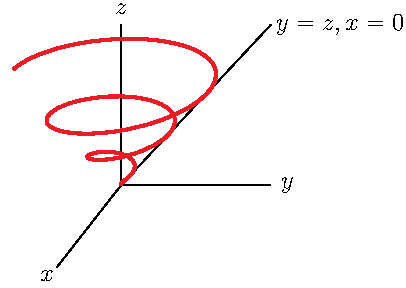
\includegraphics{corkscrew.pdf}
\end{center}
\end{efig}
By Lemma \ref{lem:CVtanArclen} 
\begin{align*}
\vr(t) &= t\cos t\,\hi + t\sin t\,\hj +t\,\hk \\
\vr'(t) &= [\cos t -t\sin t ]\hi +[\sin t+t\cos t]\hj + \hk \\
\diff{s}{t}(t)&=\big|\vr'(t)\big| \\
&= \sqrt{\big(\cos^2t-2 t\sin t\cos t +t^2\sin^2 t\big)
             +\big(\sin^2t+2 t\sin t\cos t +t^2\cos^2 t\big)+1} \\
&=\sqrt{2+t^2} 
\end{align*}
Our goal, stated at the beginning of this example, was to compute
\begin{equation*}
s(\sqrt{2})-s(0)= \int_{0}^{\sqrt{2}} \big|\vr'(t)\big|\,\dee{t}
          = \int_{0}^{\sqrt{2}} \sqrt{2+t^2}\,\dee{t}
\end{equation*}
To evaluate the integral, we'll use three techniques that you learned
in your first integral calculus course. First,  motivated by the
$\sqrt{2+t^2}$,  we'll use the trigonometric substitution
\begin{equation*}
t=\sqrt{2}\tan u\qquad
\dee{t} =\sqrt{2}\sec^2 u\,\dee{u}\qquad
2+t^2=2\big[1+\tan^2u\big]=2\sec^2 u
\end{equation*}
When $t=0$, $u=0$ and when $t=\sqrt{2}$, $\tan u=1$ so that $u=\frac{\pi}{4}$
and
\begin{align*}
s(\sqrt{2})-s(0)&= \int_{0}^{\pi/4} \sqrt{2\sec^2u}\,\sqrt{2}\sec^2 u\,\dee{u}
= 2\int_{0}^{\pi/4} \sec^3 u\,\dee{u} 
\end{align*}
You may have evaluated this integral in first year. There are several ways of doing so. Perhaps the most straight forward, but also most tedious,
method is to rewrite the integral as
\begin{equation*} 
s(\sqrt{2})-s(0)= 2\int_{0}^{\pi/4} \frac{\cos u}{\cos^4 u}\,\dee{u}
\end{equation*}
We recognize that this is a trigonometric integral that contains an odd power
of $\cos u$, so we substitute $w=\sin u$, $\dee{w}=\cos u\,\dee{u}$,
$\cos^2 u= 1-w^2$. When $u=0$, $w=0$ and when $u=\frac{\pi}{4}$, 
$w=\frac{1}{\sqrt{2}}$ so that
\begin{equation*}
s(\sqrt{2})-s(0)= 2\int_{0}^{1/\sqrt{2}}  \frac{\dee{w}}{{(1-w^2)}^2}
\end{equation*}
The integrand is now a rational function, i.e. a ratio of polynomials.
So we apply partial fractions.
\begin{align*}
s(\sqrt{2})-s(0)
&= 2\int_{0}^{1/\sqrt{2}}  \frac{\dee{w}}{{[(1-w)(1+w)]}^2} \\
&= \frac{1}{2}\int_{0}^{1/\sqrt{2}}  
        \Big[\frac{1}{1-w}+\frac{1}{1+w}\Big]^2 \dee{w} \\
&= \frac{1}{2}\int_{0}^{1/\sqrt{2}}  
        \Big[\frac{1}{(1-w)^2}+\frac{2}{(1-w)(1+w)}+\frac{1}{(1+w)^2}\Big] 
          \dee{w} \\
&= \frac{1}{2}\int_{0}^{1/\sqrt{2}}  
        \Big[\frac{1}{(1-w)^2}+\frac{1}{1-w}+\frac{1}{1+w}
             +\frac{1}{(1+w)^2}\Big]  \dee{w} \displaybreak[0]\\
&= \frac{1}{2} 
        \Big[\frac{1}{1-w}-\ln|1-w|+\ln|1+w|
             -\frac{1}{1+w}\Big]_{0}^{1/\sqrt{2}}  \\
&= \frac{1}{2} 
        \Big[\frac{2w}{1-w^2}+\ln\frac{1+w}{1-w}\Big]_{0}^{1/\sqrt{2}}  
= \frac{1}{2} 
        \Big[2\sqrt{2}+\ln\frac{\sqrt{2}+1}{\sqrt{2}-1}\Big] 
\approx 2.2956 
\end{align*}
Ooof!
\end{eg}

\section{Reparametrization}\label{sec:reparam}
There are invariably many ways to parametrize a given curve. Kind of trivially, 
one can always replace $t$ by, for example, $3u$. But there are also
more substantial ways to reparametrize curves. It often pays to tailor the parametrization used to the application of interest. For example, we shall
see in the next couple of sections that many curve formulae simplify a lot 
when arc length is used as the parameter.
\begin{eg}\label{eg:reparamCircle}
Here are three different parametrizations of the semi-circle
$x^2+y^2=r^2$, $y\ge 0$. 
\begin{itemize}\itemsep1pt \parskip0pt \parsep0pt %\itemindent-15pt
\item[$\circ$]
The first uses the polar angle $\theta$ as the parameter. We have already
seen, in Example \ref{eg:paramCircle}, the parametrization 
\begin{equation*}
\raisebox{-37pt}[37pt][30pt]{\smash{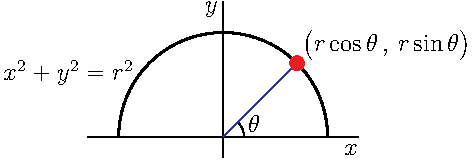
\includegraphics{reparCircleA.pdf}}}
\quad
\vr_1(\theta) = \big(r\cos\theta\,,\,r\sin\theta\big)
\qquad 0\le \theta\le \pi
\end{equation*} 

\item[$\circ$] 
The second uses $x$ as the parameter. Just solving $x^2+y^2=r^2$, $y\ge 0$
for $y$ as a function of $x$, gives $y(x) = \sqrt{r^2-x^2}$ and
so gives the parametrization
\begin{equation*}
\raisebox{-37pt}[37pt][30pt]{\smash{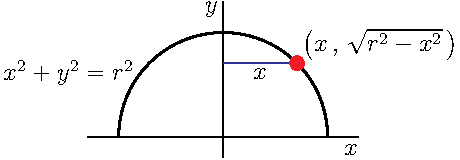
\includegraphics{reparCircleB.pdf}}}
\quad
\vr_2(x) = \big(x\,,\,\sqrt{r^2-x^2}\,\big)\qquad -r\le x\le r
\end{equation*} 

\item[$\circ$] 
The third uses arc length from $(r,0)$ as the parameter. We have seen, 
in Example \ref{eg:paramCircleTan}, that the arc length from $(r,0)$
to $\vr_1(\theta)$ is just $s=r\theta$. So the point on the semicircle 
that is arc length $s$ away from $(r,0)$ is
\begin{equation*}
\raisebox{-37pt}[37pt][30pt]{\smash{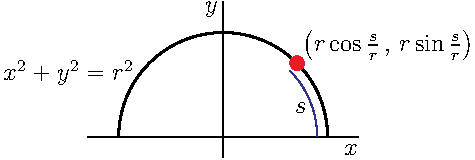
\includegraphics{reparCircleC.pdf}}}
\quad
\vr_3(s) = \vr_1\Big(\frac{s}{r}\Big) 
= \Big(r\cos\frac{s}{r}\,,\,r\sin\frac{s}{r}\Big)
%\quad
%0\le s\le \pi r
\end{equation*}
with $0\le s\le \pi r$.
\end{itemize}
\end{eg}

We shall see that, for some purposes, it is convenient to use 
parametrization by arc length.
Here is a messier example in which we reparametrize a curve so as to use
the arc length as the parameter.

\begin{eg}\label{eg:reparamAstroid}
We saw in Example \ref{eg:astroid}, that, as $t$ runs from $0$ to 
$\frac{\pi}{2}$, $\vr(t) = a \cos^3 t\,\hi+a\sin^3t\,\hj$ runs from 
$(a,0)$ to $(0,a)$ along the astroid $x^{2/3}+y^{2/3}=a^{2/3}$.
Suppose that we want a new parametrization $\vR(s)$ chosen so that, 
as $s$ runs from $0$ to some appropriate value, $\vR(s)$ runs from 
$(a,0)$ to $(0,a)$ along $x^{2/3}+y^{2/3}=a^{2/3}$, with $s$ being
the arc length from $(a,0)$ to $\vR(s)$ along $x^{2/3}+y^{2/3}=a^{2/3}$.
\begin{efig}
\begin{center}
     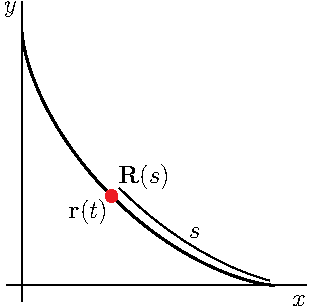
\includegraphics{astroidS.pdf}
\end{center}
\end{efig}
We saw, in Example \ref{eg:astroid}, that, for $0\le t\le \frac{\pi}{2}$, $\diff{s}{t}=\frac{3a}{2}\sin(2t)$ so that the arclength from $(a,0)=\vr(0)$ 
to $\vr(t)$ is
\begin{equation*}
s(t) = \int_0^t\frac{3a}{2}\sin(2t')\,\dee{t'} =\frac{3a}{4}\big[1-\cos(2t)\big]
\end{equation*}
which runs from $0$, at $t=0$, to $\frac{3a}{2}$, at $t=\frac{\pi}{2}$.
This is relatively clean and we can invert $s(t)$ to find $t$ 
as a function of $s$.
The value, $T(s)$, of $t$ that corresponds to any given 
$0\le s\le\frac{3a}{2}$ is determined by
\begin{equation*}
s=\frac{3a}{4}\big[1-\cos\big(2T(s)\big)\big]\qquad
\iff\qquad
T(s)=\frac{1}{2}\arccos\Big(1-\frac{4s}{3a}\Big)
\end{equation*}
and
\begin{equation*}
\vR(s) = \vr\big(T(s)\big)
       = a\cos^3\big(T(s)\big)\hi + a\sin^3 \big(T(s)\big)\hj
\end{equation*}
We can simplify $\cos^3\big(T(s)\big)$ and $\sin^3\big(T(s)\big)$
by just using trig identities to convert the  $\cos\big(2T(s)\big)$
in $s=\frac{3a}{4}\big[1-\cos\big(2T(s)\big)\big]$
into $\cos\big(T(s)\big)$'s and $\sin\big(T(s)\big)$'s.
\begin{align*}
s=\frac{3a}{4}\big[1-\cos\big(2T(s)\big)\big]
=\frac{3a}{4}\big[1-\big(2\cos^2\big(T(s)-1\big)\big]
&\iff \cos^2\big(T(s)\big)=1-\frac{2s}{3a} \\
s=\frac{3a}{4}\big[1-\cos\big(2T(s)\big)\big]
=\frac{3a}{4}\big[1-\big(1-2\sin^2\big(T(s)\big)\big]
&\iff \sin^2\big(T(s)\big)=\frac{2s}{3a}
\end{align*}
Consequently the desired parametrization is
\begin{equation*}
\vR(s) = a\left[1-\frac{2s}{3a}\right]^{3/2}\hi
        + a\left[\frac{2s}{3a}\right]^{3/2}\hj
\qquad
0\le s \le \frac{3a}{2}
\end{equation*}
which is remarkably simple.
\end{eg}

\section{Curvature}\label{sec:curvature}
So far, when we have wanted to approximate a complicated curve by
a simple curve near some point, we drew the tangent line
to the curve at the point. That's pretty crude. In particular tangent
lines are straight --- they don't curve. We will get a much better idea
of what the complicated curve looks like if we approximate it, locally,
by a very simple ``curvy curve'' rather than by a straight line.  
Probably the simplest ``curvy curve'' is a circle\footnote{Circles are good
for studying ``curvature'', because, unlike parabolas for example, the rate
at which a circle curves is uniform over the entire circle.} 
and that's what we'll use.
\begin{defn}\label{def:curvature}
\begin{enumerate}[(a)]
\item 
The circle which best approximates a given curve near a given 
point is called the \emph{circle of curvature} or the 
\emph{osculating circle}\footnote{``Osculare'' is the Latin verb ``to kiss''.
The German mathematician Gottfried Wilhelm (von) Leibniz (1646--1716)
named the circle the ``circulus osculans''.} at the point.
\item
The radius of the circle of curvature is called the \emph{radius of curvature}
at the point and is normally denoted $\rho$.
\item
The \emph{curvature} at the point is $\ka=\nicefrac{1}{\rho}$.
\item
The centre of the circle of curvature is called \emph{centre of curvature}
at the point.
\end{enumerate}
\end{defn}
\noindent
These definitions are illustrated in the figure below. It shows (part of)
the osculating circle at the point $P$. The point $C$ is the centre of
curvature. 
\begin{efig}
\begin{center}
     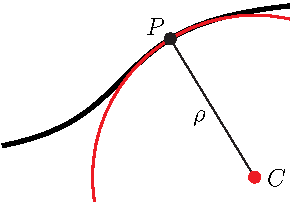
\includegraphics{curvatureDef.pdf}
\end{center}
\end{efig}


Note that when the curvature $\ka$ is large, the radius of curvature $\rho$
is small and we have a very curvy curve. On the other hand when the 
curvature $\ka$ is small, the radius of curvature $\rho$ is large and 
our curve  is almost straight. In particular, straight lines have 
curvature exactly zero.

We are now going to determine how to find the circle of curvature,
starting by figuring out what its radius should be. We'll first look 
at curves\footnote{We'll also assume that the curves of interest are smooth,
with no cusps for example, and not straight, so that the radius of 
curvature $0<\rho<\infty$.} 
that lie in the $xy$-plane and then move on to curves in 3d. 
Consider the black curve in the figure below. 
\begin{efig}
\begin{center}
     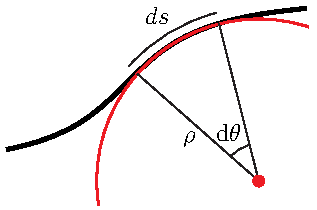
\includegraphics{curvature.pdf}
\end{center}
\end{efig}
That figure also contains a (portion of a) red circle that fits the 
curve really well between the two radial lines that are (a very small) angle
$\dee{\theta}$ apart. So the arclength $\dee{s}$ of the part of the black 
curve between the two radial lines, should be (essentially) the same 
as the arc length of the circle between the two radial lines, which is 
$\rho\,|\dee{\theta}|$, where $\rho$ is the radius of the circle. 
(We put in absolute values to take into account the
possibility that $\dee{\theta}$ could be negative.)
Thus $\dee{s} = \rho\,|\dee{\theta}|$. When $\dee{\theta}$ is a macroscopic
angle, this is of course an approximation. But in the limit as 
$\dee{\theta}\rightarrow 0$, we should end up with
\begin{equation*}
\rho = \left|\diff{s}{\theta}\right|
\end{equation*} 
We now have a formula for the radius of curvature, but not in a very 
convenient form, because to evaluate it we would need to know the arc length
along the curve as a function of the angle $\theta$ in the rightmost 
figure below.
We'll now spend some time developing more convenient formulae for $\rho$.
First consider the three figures below. They all show the same curve
as in the last figure. The leftmost figure just shows
\begin{itemize}\itemsep1pt \parskip0pt \parsep0pt %\itemindent-15pt
\item[$\circ$]
the curve of interest, which is the black curve, and
\item[$\circ$]
the (blue) point of interest on the black curve. We want to find the curvature
at that point.
\end{itemize}
The middle figure shows the same curve and point of interest and also 
shows  
\begin{itemize}\itemsep1pt \parskip0pt \parsep0pt %\itemindent-15pt
\item[$\circ$]
the red circle of curvature (i.e. best fitting circle) for the black curve 
at the blue dot.
\item[$\circ$]
The red dot is the centre of curvature.
\end{itemize}
The rightmost figure shows the same black curve, blue point of interest
and red circle of curvature (at least part of it) somewhat enlarged.
\begin{itemize}\itemsep1pt \parskip0pt \parsep0pt %\itemindent-15pt
\item[$\circ$]
The angle $\theta$ is the angle between $\hi$ and the radius
vector from the red dot (the centre of curvature) to the blue dot
(the point of interest). 
\item[$\circ$] 
$\hat\vT$ is the tangent vector to the black curve at the blue
dot. 
\item[$\circ$]  
The angle $\phi$ is the angle between $\hi$ and $\hat\vT$. 
The vector $\hat\vT$ is also tangent to the red circle. As 
the tangent and radius vectors for circles are perpendicular to 
each other\footnote{We saw that in Example \ref{eg:paramCircleTan}.}, 
we have that $\phi=\theta+\frac{\pi}{2}$ and hence 
$\rho = \big|\diff{s}{\phi}\big|$ too.
\end{itemize}
\begin{wfig}
\begin{center}
     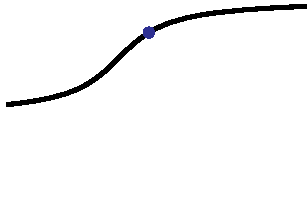
\includegraphics{curvatureB1.pdf}\hskip-20pt
     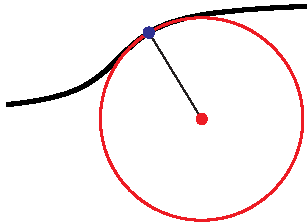
\includegraphics{curvatureB2.pdf}\qquad
     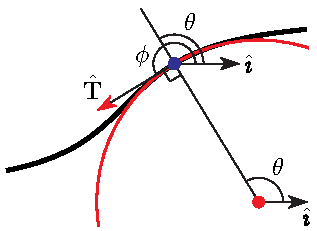
\includegraphics{curvatureB.pdf}
\end{center}
\end{wfig}
We are now in a position to develop a bunch of formulae for the radius
of curvature $\rho$ and the curvature $\ka=\frac{1}{\rho}$, that are more 
convenient than $\ka = \big|\diff{s}{\phi}\big|^{-1}$. These formulae
will use the 
\begin{notn}\label{notn:curveNotation}
If $\vr(t)$ is a parametrized curve, then
\begin{itemize}
\item 
$\vv(t) = \diff{\vr}{t}(t)$ is the velocity vector at $\vr(t)$

\item
$\va(t) = \difftwo{\vr}{t}(t) $ is the acceleration vector at $\vr(t)$

\item
$\hat\vT(t)$ is the unit tangent vector to the curve at $\vr(t)$ that
points in the direction of increasing $t$.

\item
$\hat\vN(t)$ is the unit normal vector to the curve at $\vr(t)$
that points toward the centre of curvature.

\item
$\ka(t)$ is the curvature at $\vr(t)$

\item
$\rho(t)$ is the radius of curvature at $\vr(t)$
\end{itemize}
\end{notn}

\begin{theorem}\label{thm:curvatureFormulae}

\begin{enumerate}[(a)]
\item 
Given\footnote{The equation $s=s(\phi)$ is called the ``intrinsic 
equation of the curve''.} $s(\phi)$,
i.e. if we know the arc length along the curve as a function of 
the angle\footnote{The notation $\measuredangle(\hi,\hat\vT)$
means ``the angle between $\hi$ and $\hat\vT$''.} 
$\phi=\measuredangle(\hi,\hat\vT)$, then
\begin{equation*}
\rho = \left|\diff{s}{\phi}\right|\qquad
\ka = \left|\diff{s}{\phi}\right|^{-1}\qquad
\ka = \left|\diff{\phi}{s}\right|
\end{equation*}

\item\label{thm:curvatureFormulae:part:b}
Given $\vr(s)$,
i.e. if we have a parametrization of the curve in terms of arc length, then
\begin{equation*}
\diff{\hat\vT}{s}(s) = \ka(s)\,\hat\vN(s)
\end{equation*}
where $\hat\vN(s)$ is the unit normal vector to the curve at $\vr(s)$
that points toward the centre of curvature.

\item\label{thm:curvatureFormulae:part:c}
Given $\vr(t)$, i.e. if we have a general parametrized curve,
then
\begin{align*}
\diff{\hat\vT}{t} = \ka \diff{s}{t} \hat\vN\qquad
\vv(t) =  \diff{s}{t}(t)\,\hat\vT(t) \qquad
\va(t) %= \difftwo{\vr}{t} 
       =  \difftwo{s}{t}\hat\vT
                           + \ka\left(\diff{s}{t}\right)^2\hat\vN
\end{align*}

\item 
Given $\big(x(t)\,,\,y(t)\big)$, (for curves in the $xy$-plane)
\begin{equation*}
\ka = \left|\frac{\vv(t)\times\va(t)}{\big(\diff{s}{t}\big)^3}\right|
=\frac{\big|\diff{x}{t}\difftwo{y}{t}-\diff{y}{t}\difftwo{x}{t}\big|}
{ {\big[\big(\diff{x}{t}\big)^2+\big(\diff{y}{t}\big)^2\big]}^{3/2} }
\end{equation*}

\end{enumerate}
\end{theorem}

\addtocounter{theorem}{-1}
\begin{theorem}[continued]
\begin{enumerate}[(a)]


\item[(e)]\label{thm:curvatureFormulae:part:e}
Given $y(x)$, (again for curves in the $xy$-plane)
\begin{equation*}
\ka 
=\frac{\big|\difftwo{y}{x}\big|}
{ {\big[1+\big(\diff{y}{x}\big)^2\big]}^{3/2} }
\end{equation*}

\end{enumerate}
\end{theorem}

\begin{proof}
(a) 
Given $s(\phi)$, then
\begin{equation*}
\rho = \Big|\diff{s}{\phi}\Big|\qquad
\ka = \Big|\diff{s}{\phi}\Big|^{-1}
\end{equation*}
As we are assuming that $0<\rho=\Big|\diff{s}{\phi}\Big|<\infty$, 
the inverse function theorem says that we can 
invert the function $s(\phi)$ (at least locally) to get $\phi$ as a 
function of $s$, and that
\begin{equation*}
\ka = \Big|\diff{\phi}{s}\Big|
\end{equation*}

\bigskip
\noindent (b)
Given $\vr(s)$,
then, by Lemma \ref{lem:CVtanArclen}.c, $\hat\vT(s) = \vr'(s)$ 
is a unit tangent to the curve at $\vr(s)$ and
\begin{equation}
\diff{\hat\vT}{s} = \diff{\hat\vT}{\phi} \diff{\phi}{s}
\tag{$*$}
\end{equation}
Now up to a sign $\diff{\phi}{s}$ is $\ka$, and just because 
$\phi=\measuredangle(\hi,\hat\vT)$, with $\hat\vT$ a unit vector,
\begin{equation}
\begin{split}
\hat\vT&=\cos\phi\,\hi + \sin\phi\,\hj \\
\implies \diff{\hat\vT}{\phi}&= -\sin\phi\,\hi + \cos\phi\,\hj
\end{split} 
\tag{$**$}
\end{equation}
So $\diff{\hat\vT}{\phi}$ is a unit vector that is 
perpendicular\footnote{Think about why this should be the case. In particular,
sketch $\hat\vT$ and $\phi$ and think about what the sketch says about 
$\diff{\hat\vT}{\phi}$.} to $\hat\vT$, and hence to the curve at $\vr(s)$, and
\begin{equation}
\diff{\hat\vT}{s}(s) = \ka(s)\,\hat\vN(s)
\tag{$\dagger$}
\end{equation}
with $\hat\vN(s)$ a unit normal vector to the curve at $\vr(s)$.
In fact, $\hat\vN(s)$ is the unit normal vector to the curve at $\vr(s)$
that points toward the centre of curvature.

To see that,
look at the figures below\footnote{In each of the four figures, the arrow on the curve specifies the direction of increasing arc length $s$ and 
the red dot is the centre of curvature for the curve at the blue dot.}, 
and note that substituting the sign information
from each figure into ($*$) gives ($\dagger$).
For example,
\vadjust{
\begin{efig}
\begin{center}
     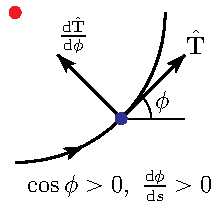
\includegraphics{curvatureSignA.pdf}\qquad\qquad\quad
     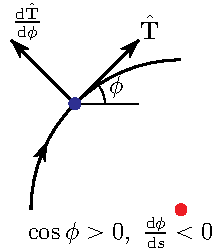
\includegraphics{curvatureSignC.pdf}
\end{center}
\begin{center}
     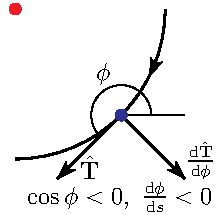
\includegraphics{curvatureSignB.pdf}\qquad\qquad\quad
     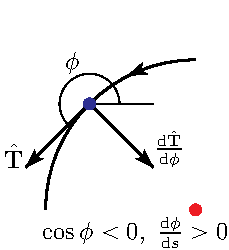
\includegraphics{curvatureSignD.pdf}
\end{center}
\end{efig}
}
consider the figure on the lower left. In that figure,
\begin{itemize}\itemsep1pt \parskip0pt \parsep0pt %\itemindent-15pt
\item[$\circ$] 
the $x$ component of $\hat\vT$ is negative ($\hat\vT$ is leftward pointing in the figure),
\begin{itemize}\itemsep1pt \parskip0pt \parsep0pt %\itemindent-15pt
\item[$\circ$] 
which makes $\cos\phi$ negative (see ($**$)), 
\item[$\circ$] 
which makes the $y$ component of $\diff{\hat\vT}{\phi}$ negative
            (see ($**$) again),
\item[$\circ$] 
so $\diff{\hat\vT}{\phi}$ is downward pointing,
\end{itemize}
so $\diff{\hat\vT}{\phi}=-\hat\vN$ (the centre of curvature is the red dot 
above the curve) and
\item[$\circ$] as $s$ increases (i.e. as you move in the direction of the
arrow on the curve), $\phi$ decreases (on the far right hand part of the curve $\phi\approx\frac{3\pi}{2}$, while on the far left hand part of the curve $\phi\approx\pi$), so $\diff{\phi}{s}<0$ and
$\ka = \big|\diff{\phi}{s}\big| = - \diff{\phi}{s}$.
\item[$\circ$] So by ($*$),
$\diff{\hat\vT}{s} = \diff{\hat\vT}{\phi} \diff{\phi}{s}
=\big(-\hat\vN)(-\ka) = \ka\hat\vN$.
\end{itemize}
In each of the three other figures we also end up with 
$\diff{\hat\vT}{s} = \ka(s)\hat\vN(s)$.
\intremark{
We are assuming that $\ka>0$ so that $\diff{\phi}{s}\ne 0$, and we have either
\begin{itemize}\itemsep1pt \parskip0pt \parsep0pt %\itemindent-15pt
\item[$\circ$] 
$\diff{\phi}{s}>  0$ in which case $\ka=\diff{\phi}{s}$ or
\item[$\circ$] 
$\diff{\phi}{s}<  0$ in which case $\ka=-\diff{\phi}{s}$ or
\end{itemize}
and we also have either
\begin{itemize}\itemsep1pt \parskip0pt \parsep0pt %\itemindent-15pt
\item[$\circ$] 
$\cos\phi >  0$ in which case $\diff{\hat\vT}{\phi}$ is upward pointing or
\item[$\circ$] 
$\cos\phi <  0$ in which case $\diff{\hat\vT}{\phi}$ is downward pointing or
\item[$\circ$] 
$\cos\phi = 0$, $\sin\phi>0$ in which case $\diff{\hat\vT}{\phi}$ is leftward pointing or
\item[$\circ$] 
$\cos\phi = 0$, $\sin\phi<0$ in which case $\diff{\hat\vT}{\phi}$ is rightward pointing.
\end{itemize}
The four figures cover all cases in which $\cos\phi\ne 0$. The remaining
four (nongeneric) cases with $\cos\phi$ could be handled by similar 
pictures, or by continuity.

}

\noindent
Note that if $\ka(s)=0$, then $\hat\vN(s)$ is not defined. This makes sense:
if the curve is (locally) a straight line, there is no ``best fitting circle''.

\bigskip
\noindent (c)
Given $\vr(t)$,
i.e. if we have a general parametrized curve, we can determine a unit
tangent vector by using Lemma \ref{lem:CVtanArclen}:
\begin{equation*}
\vv(t) = \diff{\vr}{t}(t) = \diff{s}{t}(t)\,\hat\vT(t)
\quad\implies\quad
\hat\vT(t) = \frac{\vr'(t)}{|\vr'(t)|}
\end{equation*}
Then we can determine $\ka$ and $\hat\vN$  by differentiating
$\hat\vT(t)$ and using the chain rule:
\begin{equation*}
\diff{\hat\vT}{t} = \diff{\hat\vT}{s}\diff{s}{t}
 = \ka \diff{s}{t} \hat\vN
\quad\implies\quad
\ka(t) = \frac{|\hat\vT'(t)|}{|\vr'(t)|}
\end{equation*}
Also, if we differentiate $\vv(t) = \diff{s}{t}\hat\vT(t)$, we get
that the acceleration
\begin{equation*}
\va(t) = \difftwo{\vr}{t} 
       =  \difftwo{s}{t}\hat\vT + \diff{s}{t}\,\diff{\hat\vT}{t}
       =  \difftwo{s}{t}\hat\vT
                           + \ka\Big(\diff{s}{t}\Big)^2\hat\vN
\end{equation*}

\bigskip
\noindent (d)\label{clpcurvesthm:curvatureFormulae:partd}
Given $\big(x(t)\,,\,y(t)\big)$, (for curves in the $xy$-plane),
we can read off the curvature from
\begin{align*}
\vv(t)\times\va(t) 
&=\Big(\diff{s}{t}(t)\,\hat\vT(t)\Big)\times
    \Big(\difftwo{s}{t}\hat\vT
                           + \ka\Big(\diff{s}{t}\Big)^2\hat\vN\Big) 
\\
&= \ka\Big(\diff{s}{t}\Big)^3\hat\vT\times\hat\vN
\qquad\text{(since $\hat\vT\times\hat\vT=\vZero$)}
\end{align*} 
Think of $\hat\vT$ and $\hat\vN$ as 3d vectors that whose $z$-components happen to be zero. As $\hat\vT$ and $\hat\vN$ are mutually perpendicular 
unit vectors in the $xy$-plane, the cross-product $\hat\vT\times\hat\vN$
will be either $+\hk$ or $-\hk$. In both cases, 
$|\vv(t)\times\va(t)\big| = \ka\big|\diff{s}{t}\big|^3$. So
\begin{align*}
\ka &= \left|\frac{\vv(t)\times\va(t)}{\big(\diff{s}{t}\big)^3}\right|
=\left|\frac{\big[\diff{x}{t}\hi+\diff{y}{t}\hj\big]\times
        \big[\difftwo{x}{t}\hi+\difftwo{y}{t}\hj\big]}
           {\big(\diff{s}{t}\big)^3}\right|
=\left|\frac{\big[\diff{x}{t}\difftwo{y}{t}-\diff{y}{t}\difftwo{x}{t}\big]\hk}
           {\big(\diff{s}{t}\big)^3}\right|
\\
&=\frac{\big|\diff{x}{t}\difftwo{y}{t}-\diff{y}{t}\difftwo{x}{t}\big|}
{ {\big[\big(\diff{x}{t}\big)^2+\big(\diff{y}{t}\big)^2\big]}^{3/2} }
\end{align*}

\bigskip
\noindent (e)
Given $y(x)$, again for curves in the $xy$-plane,
we can parametrize the curve using $x$ as the parameter:
\begin{equation*}
\vr(t) = \big(X(t)\,,\,Y(t)\big) \qquad\text{with $X(t)=t$ and $Y(t) =y(t)$}
\end{equation*}
Then
\begin{equation*}
\diff{X}{t} = 1 \qquad
\difftwo{X}{t} = 0 \qquad
\diff{Y}{t} = \diff{y}{x} \qquad
\difftwo{Y}{t} = \difftwo{y}{x}
\end{equation*}
and 
\begin{equation*}
\ka 
=\frac{\big|\diff{X}{t}\difftwo{Y}{t}-\diff{Y}{t}\difftwo{X}{t}\big|}
{ {\big[\big(\diff{X}{t}\big)^2+\big(\diff{Y}{t}\big)^2\big]}^{3/2} }
=\frac{\big|\difftwo{y}{x}\big|}
{ {\big[1+\big(\diff{y}{x}\big)^2\big]}^{3/2} }
\end{equation*}
\end{proof}

\noindent
Take another look at Theorem \ref{thm:curvatureFormulae}.c 
and note that
\begin{itemize}\itemsep1pt \parskip0pt \parsep0pt %\itemindent-15pt
\item[$\circ$] 
the tangential component of acceleration, i.e. $\difftwo{s}{t}$,
arises purely from change in speed while
\item[$\circ$] 
the normal component of acceleration, i.e. $\ka\big(\diff{s}{t}\big)^2$,
arises from curvature and is proportional to the square of the speed
$\diff{s}{t}$. Think about what you feel when you are driving.
That's why velodromes and (car) race tracks often have banked corners.

\end{itemize}



\begin{eg}\label{eg:curveCircle}
As a warm up example, and also a check that our formulae make sense,
we'll find the curvature $\ka$, radius of curvature, $\rho$, unit tangent
vector, $\hat\vT$, unit normal vector, $\hat\vN$, and centre of curvature 
of the parametrized curve
\begin{equation*}
\vr(t) = a\cos t\,\hi + a\sin t\,\hj
\end{equation*}
with the constant $a>0$.
This is, of course, the circle of radius $a$ centred on the origin.
As
\begin{equation*}
\vv(t)=\diff{\vr}{t}(t)= -a\sin t\,\hi + a\cos t\,\hj
\implies \diff{s}{t}(t) = |\vv(t)| = a
\end{equation*}
we have that the unit tangent vector
\begin{equation*}
\vT(t) = \frac{\vv(t)}{|\vv(t)|} = -\sin t\,\hi + \cos t\,\hj
\end{equation*}
Note, as a check, that this is indeed a vector of length one and
is perpendicular to the radius vector (as expected --- the curve is a circle).
As 
\begin{equation*}
\diff{\hat\vT}{t}(t)= -\cos t\,\hi  -\sin t\,\hj
\end{equation*}
we have that
\begin{equation*}
\hat\vN(t) = \frac{\diff{\hat\vT}{t}(t)}{\big|\diff{\hat\vT}{t}(t)\big|}
           = -\cos t\,\hi  -\sin t\,\hj
\quad
\ka(t) 
= \frac{\big|\diff{\hat\vT}{t}(t)\big|}{\diff{s}{t}(t)}
=\frac{1}{a}
\quad
\rho(t)=\frac{1}{\ka(t)} =a
\end{equation*}
Now look at the figure.
\begin{efig}
\begin{center}
     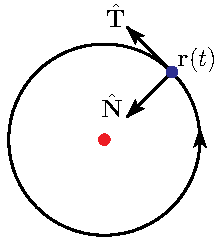
\includegraphics{circleCentreB.pdf}
\end{center}
\end{efig}
To get to the centre of curvature we should start from
$\vr(t)$ and walk a distance $\rho(t)$, which after all is the radius
of curvature, in the direction $\hat\vN(T)$, which is pointing towards the centre of curvature. So the centre of curvature is
\begin{equation*}
\vr(t)+\rho(t)\hat\vN(t) 
=\big[a\cos t\,\hi  +a\sin t\,\hj\big]
+a\big[-\cos t\,\hi  -\sin t\,\hj\big]
= \vZero
\end{equation*}
This makes perfectly good sense --- the radius of curvature is
the radius of the original circle and the centre of curvature is the
centre of the original circle.


One alternative calculation of the curvature, using $x(t) = a\cos t $,
$y(t)=a\sin t$, is
\begin{align*}
\ka(t)
&=\frac{\big|
  \diff{x}{t}(t)\difftwo{y}{t}(t)-\diff{y}{t}(t)\difftwo{x}{t}(t)
  \big|}{\Big[\big(\diff{x}{t}(t)\big)^2
                +\big(\diff{y}{t}(t)\big)^2\Big]^{3/2}} \\
&=\frac{\big|
  -a\sin t\big(-a\sin t\big)-a\cos t\big(-a\cos t\big)
  \big|}{\big[\big(-a\sin t\big)^2
                +\big(a\cos t\big)^2\big]^{3/2}} \\
&=\frac{1}{a}
\end{align*}
Another alternative calculation of the curvature, using $y(x) 
=\sqrt{a^2-x^2}$ (for the part of the circle with $y>0$),
\begin{equation*}
y'(x) = -\frac{x}{\sqrt{a^2-x^2}}=-\frac{x}{y(x)} \qquad
y''(x) = -\frac{y(x) - xy'(x)}{y(x)^2}
       =  -\frac{y(x)^2 + x^2}{y(x)^3}
       =  -\frac{a^2}{y(x)^3}
\end{equation*}
is 
\begin{align*}
\ka(x)
&=\frac{\big|\difftwo{y}{x}(x)\big|}
  {\Big[1+\big(\diff{y}{x}(x)\big)^2\Big]^{3/2}} 
=\frac{\frac{a^2}{y(x)^3}}
  {\Big[1+\frac{x^2}{y(x)^2}\Big]^{3/2}}
=\frac{a^2}{\big[y(x)^2+x^2\big]^{3/2}}
=\frac{1}{a}
\end{align*}
\end{eg}



\begin{eg}\label{eg:curvatureEtc}
As a more computationally involved example, we'll analyze
\begin{align*}
\vr(t) &= \big(\cos t + t\sin t\big)\hi +\big(\sin t-t\cos t\big)\hj
\qquad t>0 \\
\vv(t) &= t\cos t\,\hi + t\sin t\,\hj \\
\va(t) &= \big(\cos t - t\sin t\big)\hi +\big(\sin t+t\cos t\big)\hj 
\end{align*}
We can read off from $\vv(t)$, that
\begin{align*}
\diff{s}{t}(t) &= |\vv(t)| =t \\
\difftwo{s}{t}(t) &= 1 \\
\vT(t)&=\frac{\vv(t)}{|\vv(t)|} = \cos t\,\hi + \sin t\,\hj
\end{align*}
Next, from $\va(t)$, we read off that
\begin{align*}
\va(t) &=\big(\cos t - t\sin t\big)\hi +\big(\sin t+t\cos t\big)\hj\qquad
\text{and}  \\
\va(t)&=\difftwo{s}{t}(t)\,\hat\vT(t)
                             +\ka(t)\left(\diff{s}{t}(t)\right)^2\hat\vN(t)
\qquad\text{(by Theorem \ref{thm:curvatureFormulae}.c)} \\
&=\cos t\,\hi + \sin t\,\hj +t^2\ka(t) \hat\vN(t) \\
\implies 
t^2\ka(t) \hat\vN(t)&= - t\sin t\,\hi + t\cos t\,\hj
\end{align*}
so that $t^2\ka(t)$ is the length of $- t\sin t\,\hi + t\cos t\,\hj$, which is $t$. Thus
\begin{align*}
\ka(t) = \frac{1}{t} \quad\text{and}\quad
\hat\vN(t)= \frac{- t\sin t\,\hi + t\cos t\,\hj}{t^2\ka(t)} 
          = -\sin t\,\hi + \cos t\,\hj
\end{align*}
As an alternative calculation of the curvature, we have
\begin{align*}
\ka(t)
&=\frac{|\vv(t)\times\va(t)|}{(\diff{s}{t}(t))^3} \\
&=\frac{\big|\big[t\cos t\,\hi + t\sin t\,\hj\big]\times
      \big[\big(\cos t - t\sin t\big)\hi +\big(\sin t+t\cos t\big)\hj\big]\big|}
{(\diff{s}{t}(t))^3} \\
&=\frac{\big|\big[t\cos t\big(\sin t+t\cos t\big)
                 -t\sin t\big(\cos t - t\sin t\big)\big]\hk\big|}
{(\diff{s}{t}(t))^3} \\
&=\frac{|t^2\hk|}{t^3}
=\frac{1}{t}
\end{align*}
It pays to think before you calculate!
\end{eg}

\section{Curves in Three Dimensions}\label{sec:Curve3d}
So far, we have developed formulae for the curvature, unit tangent vector,
etc., at a point $\vr(t)$ on a curve that lies in the $xy$-plane. We 
now extend our discussion to curves in $\bbbr^3$. Fix any $t$.
For $t'$ very close to $t$, $\vr(t')$, will, by the Taylor expansion 
to second order, be very close to $\vr(t) + \vr'(t)\,(t'-t) 
+\frac{1}{2}\vr''(t)\,(t'-t)^2$, so that $\vr(t')$ almost lies in the 
plane through $\vr(t)$ that is determined by the two vectors $\vr'(t)$ and 
$\vr''(t)$. Thus, if we restrict
our attention to a very small part of the curve near the point of 
interest $\vr(t)$, the curve will, to a very good approximation lie in 
some plane. So we can still define, for example, the osculating circle 
to the curve at $\vr(t)$ to be the circle in that plane that fits the 
curve best near $\vr(t)$. And we still have the formulae\footnote{The arguments in the proof of Theorem \ref{thm:curvatureFormulae} that we used to verify 
these formulae work in any plane, not just the $xy$-plane. Just choose 
$\hi$ and $\hj$ to be any two mutually perpendicular unit vectors in the plane.}
\begin{align*}
\vv&=\diff{\vr}{t}=\diff{s}{t}\,\hat\vT\\
\diff{\hat\vT}{s} &= \ka\hat\vN\\
\diff{\hat\vT}{t} &= \ka\diff{s}{t}\hat\vN\\
\va&=\difftwo{\vr}{t}=\difftwo{s}{t}\,\hat\vT
                             +\ka\Big(\diff{s}{t}\Big)^2\hat\vN\\
\vv\times\va &= \ka \Big(\diff{s}{t}\Big)^3\hat\vT\times\hat\vN
\end{align*}
The only\footnote{However this can be a significant difference.} 
difference is that $\vv$, $\va$, $\hat\vT$ and $\hat\vN$
are now three component vectors rather than two component vectors. 

If we are lucky and our curve happens to lie completely in a single plane, 
the vectors $\hat\vT(s)$ and $\hat\vN(s)$ are mutually perpendicular 
unit vectors that lie in the same plane, so that their cross product
$\hat\vB(s) = \hat\vT(s)\times\hat\vN(s)$
is a unit vector that is perpendicular to the plane.  By continuity, 
$\hat\vB(s)$ has to be a constant vector, i.e. be independent of $s$. 

If, on the other hand, $\hat\vB(s)$ is not constant, then our curve 
doesn't lie  in a single plane, and we can use the derivative
\begin{align*}
\diff{\hat\vB}{s}
&=\diff{ }{s}\big(\hat\vT\times\hat\vN\big)
=\diff{\hat\vT}{s}\times\hat\vN + \hat\vT\times \diff{\hat\vN}{s} \\
&=\hat\vT\times \diff{\hat\vN}{s}\qquad
\text{$\Big($since $\diff{\hat\vT}{s}$ is parallel to $\hat\vN$$\Big)$}
\end{align*} 
as a measure
\begin{itemize}\itemsep1pt \parskip0pt \parsep0pt \itemindent 15pt
\item[$\circ$]
of how badly the curve fails to lie in a plane, 
\item[$\circ$] i.e. how much the
plane that fits the curve best near $\vr(s)$ twists as $s$ increases,
\end{itemize}
The cross product in $\diff{\hat\vB}{s}=\hat\vT\times \diff{\hat\vN}{s}$ 
implies that $\diff{\hat\vB}{s}$ is perpendicular to $\hat\vT$. In addition,
$\diff{\hat\vB}{s}$ must be perpendicular to $\hat\vB$ because
\begin{equation*}
|\hat\vB|=1
\implies 1=\hat\vB\cdot\hat\vB
\implies 0 = \diff{}{s}\left[\hat\vB\cdot\hat\vB\right]
          = 2 \hat\vB\cdot\diff{\hat\vB}{s}
\end{equation*}
So $\diff{\hat\vB}{s}(s)$ must be parallel to $\hat\vN(s)$.

\begin{defn}\label{def:torsion}
\begin{enumerate}[(a)]
\item The \emph{binormal vector} at $\vr(s)$ is 
$\hat\vB(s) = \hat\vT(s)\times \hat\vN(s)$. 
The normal vector $\hat\vN(s)$ is sometimes called the unit
\emph{principal normal vector} to distinguish it from the
binormal vector.

\item
 We define the \emph{torsion}
$\tau(s)$ by
\begin{equation*}
\diff{\hat\vB}{s}(s) = -\tau(s)\hat\vN(s)
\end{equation*}
The negative sign is included so that $\tau(s)>0$ indicates
``right handed twisting''. There will be an explanation of what this means in Example \ref{eg:helixTwist} below.
\item
The \emph{osculating plane} at $\vr(s)$ (the plane that fits the curve best 
at $\vr(s)$) is the plane through $\vr(s)$ with normal vector $\hat\vB(s)$.
The equation of the plane is
\begin{equation*}
\hat\vB(s)\cdot\big\{(x,y,z)-\vr(s)\big\}=0
\end{equation*}
\end{enumerate}
\end{defn}

For each $s$, $\hat\vT(s)$, $\hat\vN(s)$ and $\hat\vB(s)$ are mutually
perpendicular unit vectors. They form an orthonormal basis
for $\bbbr^3$, just as $\hi$, $\hj$ and $\hk$ form an orthonormal basis
for $\bbbr^3$. Furthermore both $(\hat\vT(s)\,,\,\hat\vN(s)\,,\,\hat\vB(s))$ 
and $(\hi\,,\,\hj\,,\,\hk)$ are ``right handed triples\footnote{We shall
stick to ``right handed triples'' to make it easier to get various signs right.}'',
meaning that $\hat\vB(s) = \hat\vT(s)\times\hat\vN(s)$ and $\hk=\hi\times\hj$.


\begin{efig}
\begin{center}
     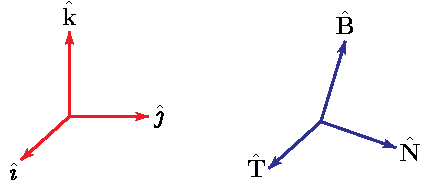
\includegraphics{cross.pdf}
\end{center}
\end{efig}

We have already computed $\diff{\hat\vT}{s}$ and $\diff{\hat\vB}{s}$.
It is now an easy matter to compute
\begin{align*}
\diff{\hat\vN}{s} 
&= \diff{}{s}\big(\hat\vB(s)\times\hat\vT(s)\big)\\
&= -\tau(s)\hat\vN(s)\times\hat\vT(s)
  +\hat\vB(s)\times\big(\ka(s)\hat\vN(s)\big) \\
&=\tau(s)\hat\vB(s)-\ka(s)\hat\vT(s)
\end{align*}
To see that $\hat\vN(s)\times\hat\vT(s)=-\hat\vB(s)$ and
$\hat\vB(s)\times\hat\vN(s)=-\hat\vT(s)$, just look at the right hand figure above.


Now suppose that we have a curve that is parametrized by $t$ rather than $s$.
How do we find the torsion $\tau$? The most obvious method is to
\begin{itemize}
\item
recall that $\vv\times\va = \ka \big(\diff{s}{t}\big)^3\hat\vT\times\hat\vN
                          = \ka \big(\diff{s}{t}\big)^3\hat\vB$
and that $\hat\vB(t)$ is a unit vector. So
\begin{equation*}
\hat\vB(t) = \frac{\vv(t)\times\va(t)}{|\vv(t)\times\va(t)|}
\end{equation*}

\item Having found $\vB(t)$ we can differentiate it and use
$\diff{\hat\vB}{s}(s) = -\tau(s)\hat\vN(s)$ and the chain rule to give
\begin{equation*}
\diff{\vB}{t} = \diff{\vB}{s}\diff{s}{t} = -\tau\diff{s}{t} \hat\vN
\end{equation*}
from which we can read off $\tau$, provided we know $\diff{s}{t}$ and
$\hat\vN$.

\end{itemize}


There is another, often more efficient, method to find the torsion $\tau$ 
that uses
\begin{align*}
\diff{\va}{t} &= \diff{}{t}\Big(\difftwo{s}{t}\,\hat\vT
                             +\ka\Big(\diff{s}{t}\Big)^2\hat\vN\Big) \\
       &= \ddiff{3}{s}{t}\,\hat\vT
         +\difftwo{s}{t}\,\diff{s}{t}\,\ka\hat\vN
         +\diff{}{t}\Big(\ka\Big(\diff{s}{t}\Big)^2\Big)\hat\vN
         +\ka\Big(\diff{s}{t}\Big)^3
               \big(\tau\hat\vB-\ka\hat\vT\big)
\end{align*}
While this looks a little complicated, notice that, with just 
one exception, namely 
$\ka\big(\diff{s}{t}\big)^3\tau(s)\hat\vB(s)$, every term on the right 
hand side is either in the direction $\hat\vT$ or in the direction 
$\hat\vN$ and so is perpendicular to $\hat\vB$. So, dotting with 
$\vv\times\va = \ka \big(\diff{s}{t}\big)^3\hat\vB$ gives
\begin{align*}
\big(\vv\times\va\big)\cdot \diff{\va}{t} 
   = \ka^2 \Big(\diff{s}{t}\Big)^6\,\tau
   = |\vv\times\va|^2\,\tau
\end{align*}
and hence
\begin{align*}
\tau = \frac{\big(\vv\times\va\big)\cdot \diff{\va}{t} }{|\vv\times\va|^2}
\end{align*}


If the curvature\footnote{As in two dimensions, if $\ka(s)=0$, then
$\hat\vN(s)$ is not defined. This makes even more sense in three dimensions
than in two dimensions: if the curve is a straight line, there are 
infinitely many unit vectors perpendicular to it and there is no way to 
distinguish between them.} $\ka(s)>0$ 
and the torsion $\tau(s)$ are known,
then the system of equations\footnote{The equations are named after 
the two French mathematicians who independently discovered them: 
Jean Fr\'ed\'eric Frenet (1816--1900, the son of a wig maker), 
in his thesis of 1847
(actually he only gave two of the three equations), and 
Joseph Alfred Serret (1819--1885) in 1851. 
%One of the universities that Serret atended was the \'Ecole tabac.
}
\begin{impeqn}[Frenet--Serret Formulae]\label{eqn:FrenetSerret}
\begin{align*}
\diff{\hat\vT}{s}(s)&=\phantom{-}\ka(s)\ \hat\vN(s)\cr
\diff{\hat\vN}{s}(s)&=\phantom{-}\tau(s)\ \hat\vB(s)-\ka(s)\ \hat\vT(s)\cr
\diff{\hat\vB}{s}(s)&=-\tau(s)\ \hat\vN(s)\cr
\end{align*}
\end{impeqn}\noindent
is a first order linear system of ordinary differential equations 
\begin{align*}
\diff{}{s}
\left[ \begin{matrix}\hat\vT(s)\\ \hat\vN(s)\\ \hat\vB(s)\end{matrix} \right]
=\left[\begin{matrix} 0      & \ka(s) & 0\\
              -\ka(s) &  0     &\tau(s) \\
              0       &-\tau(s)  & 0 \end{matrix}\right]
\left[\begin{matrix}\hat\vT(s)\\ \hat\vN(s)\\ \hat\vB(s)\end{matrix}\right]
\end{align*}
for the $9$ component vector valued function
$(\hat\vT(s)\,,\,\hat\vN(s)\,,\,\hat\vB(s))$. 

Any first order linear initial 
value problem
\begin{equation*}
\diff{}{s}\vx(s) = M(s) \vx(s)\qquad
\vx(0)=\vx_0
\end{equation*}
where $\vx$ is an $n$-component vector and $M(s)$ is an $n\times n$ matrix with continuous entries, has exactly one solution. If $n=1$, so that 
$\vx(s)$ and $M(s)$ are just functions, this is easy to see. Just 
let $\cM(s)$ be the antiderivative of $M(s)$ that obeys $\cM(0)=0$. Then
\begin{align*}
\diff{}{s}\vx(s) = M(s) \vx(s)
&\iff e^{-\cM(s)}\diff{}{s}\vx(s) - M(s) e^{-\cM(s)} \vx(s)=0 \\
&\iff \diff{}{s}\Big(e^{-\cM(s)}\vx(s)\Big) = 0
\end{align*}
by the product rule. So $e^{-\cM(s)}\vx(s)$ is a constant independent of $s$. 
In particular $e^{-\cM(s)}\vx(s)=e^{-\cM(0)}\vx(0)= \vx_0$ so that 
 $\vx(s) = \vx_0 e^{\cM(s)}$.
This argument can be generalized to any natural number $n$. But that is 
beyond the scope of this book.


Since the Frenet-Serret formulae constitute a first order system of ordinary
differential equations for the vector 
$(\hat\vT(s)\,,\,\hat\vN(s)\,,\,\hat\vB(s))$ and since any first order linear 
initial value problem has a exactly one solution,
\begin{itemize}\itemsep1pt \parskip0pt \parsep0pt %\itemindent-15pt
\item[$\circ$] 
the vector valued function $(\hat\vT(s)\,,\,\hat\vN(s)\,,\,\hat\vB(s))$ 
is determined by the functions
$\ka(s)$ and $\tau(s)$ (assuming that they are continuous) together with 
the initial condition $(\hat\vT(0)\,,\,\hat\vN(0)\,,\,\hat\vB(0))$.
\item[$\circ$] Furthermore, once you know $\hat\vT(s)$, then
$\vr(s)$ is determined by $\vr(0)$ and $\diff{\vr}{s}(s)=\hat\vT(s)$.
\item[$\circ$] So any smooth curve $\vr(s)$ is completely determined
by $\vr(0)$, $(\hat\vT(0)\,,\,\hat\vN(0)\,,\,\hat\vB(0))$, $\ka(s)$
and $\tau(s)$. 
\item[$\circ$] That is, up to translations (you can move between any two 
possible choices of $\vr(0)$ by  a translation) and rotations
(you can move between any two possible choices of 
$(\hat\vT(0)\,,\,\hat\vN(0)\,,\,\hat\vB(0))$ by  a rotation) a curve is       completely determined by the curvature $\ka(s)>0$ and the torsion 
$\tau(s)$. This result is called ``The fundamental theorem of space curves''.

\end{itemize}

\begin{theorem}[The Fundamental Theorem of Space Curves]
Let $\ka(s)>0$ and $\tau(s)$ be continuous. Then up to translations
and rotations, there is a unique curve with curvature $\ka(s)$ and
torsion $\tau(s)$.
\end{theorem}

\begin{eg}[Right circular helix]\label{eg:helixTwist}
The right circular helix is the curve
\begin{align*}
\vr(t)= a\cos t\,\hi +a\sin t\,\hj + bt\,\hk
\end{align*}
with $a,b>0$ as in the figure on the left below. 
\begin{efig}
\begin{center}
    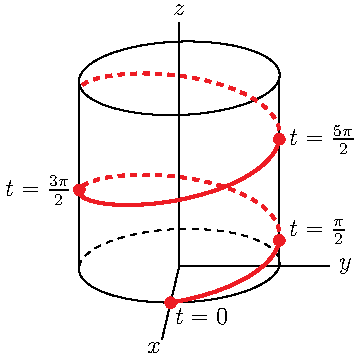
\includegraphics{helix5.pdf} \qquad
   % \raisebox{0.5\height}{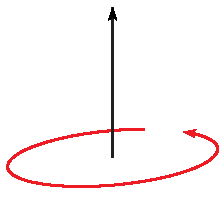
\includegraphics[scale=1.0]{helix3.pdf}}\qquad
%    \raisebox{0.1\height}{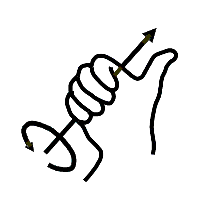
\includegraphics[scale=1.5]{Right-hand_rule.pdf}}
    \raisebox{0.4\height}{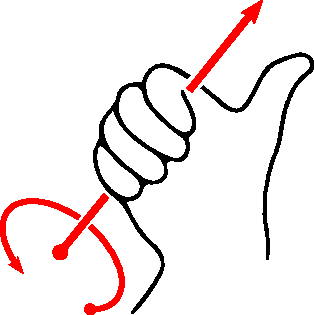
\includegraphics[scale=0.7]{RHR.pdf}}
\end{center}
\end{efig}
Here is why it is called a \emph{right} helix 
rather than a left helix. If the helix is the thread of a bolt that you 
are screwing into a nut, and you turn the bolt in the direction of the 
(curled) fingers of your right hand 
%(as in the red circle of the figure on the right above), 
(as in the figure\footnote{This figure is a variant of 
https:/\hskip-1pt/commons.wikimedia.org/wiki/File:Right\_hand\_rule\_simple.png
} on the right above), 
then it moves in the direction of your thumb (as 
in the long straight arrow of the figure on the right above). 

To determine the curvature and torsion of this curve we compute
\begin{align*}
\vv(t)&= -a\sin t\,\hi +a\cos t\,\hj + b\,\hk  \\
\va(t)&= -a\cos t\,\hi -a\sin t\,\hj \\
\diff{\va}{t}(t)&= a\sin t\,\hi -a\cos t\,\hj
\end{align*}
From $\vv(t)$ we read off
\begin{align*}
\diff{s}{t}=\sqrt{a^2+b^2}\qquad
\hat\vT(t)= -\frac{a}{\sqrt{a^2+b^2}}\sin t\,\hi
           +\frac{a}{\sqrt{a^2+b^2}} \cos t\,\hj
           +\frac{b}{\sqrt{a^2+b^2}}\,\hk
\end{align*}
From $\va=\difftwo{s}{t}\,\hat\vT+\ka\big(\diff{s}{t}\big)^2\hat\vN
=\ka(a^2+b^2)\hat\vN$, we read off that
\begin{align*}
\ka(t)=\frac{a}{a^2+b^2}\qquad
\hat\vN(t) = -\cos t\,\hi-\sin t\,\hj
\end{align*}
From
\begin{align*}
\vv(t)\times\va(t)  &= \det\left[
                \begin{matrix}  \hi   & \hj     & \hk \\
                             -a\sin t & a\cos t &  b \\
                             -a\cos t &-a\sin t & 0\end{matrix} \right] 
         = ab\sin t\,\hi -ab\cos t\,\hj +a^2\,\hk \\
|\vv(t)\times\va(t)|^2 &=a^2b^2+a^4 = a^2(a^2+b^2)
\end{align*}
we read off
\begin{align*}
\hat\vB(t) & = \frac{\vv(t)\times\va(t)}{|\vv(t)\times\va(t)|}
= \frac{b}{\sqrt{a^2+b^2}}\sin t\,\hi
           -\frac{b}{\sqrt{a^2+b^2}} \cos t\,\hj
           +\frac{a}{\sqrt{a^2+b^2}}\,\hk
\end{align*}
and
\begin{align*}
\tau(t) & = \frac{\big(\vv\times\va\big)\cdot \diff{\va}{t} }{|\vv\times\va|^2}
=\frac{a^2b}{a^2(a^2+b^2)}
=\frac{b}{a^2+b^2}
\end{align*}
Note that, for the right handed helix, $\tau>0$. Finally the centre of 
curvature is
\begin{align*}
\vr(t) +\frac{1}{\ka(t)}\hat\vN(t)
&=\Big(a-\frac{a^2+b^2}{a}\Big)\cos t\,\hi
 +\Big(a-\frac{a^2+b^2}{a}\Big)\sin t\,\hi
 +bt\,\hk \\
&=-\frac{b^2}{a}\cos t\,\hi
  -\frac{b^2}{a}\sin t\,\hi
 +bt\,\hk 
\end{align*}
which is another helix. In the figure below, the red curve is the original
helix and the blue curve is the helix traced by the centre of curvature.
\begin{nfig}
\begin{center}
    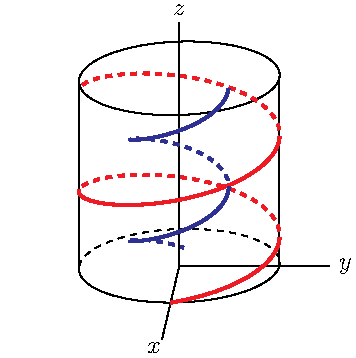
\includegraphics{helix6.pdf}
\end{center}
\end{nfig}

\end{eg}



\section{A Compendium of Curve Formula}\label{sec:CurveCompendium}

In the following $\vr(t)=\big(x(t)\,,\,y(t)\,,\,z(t)\big)$ 
is a parametrization of some curve. The vectors $\hat\vT(t),\ \hat\vN(t),\ $ 
and $\ \hat\vB(t)\ $ are the unit tangent,
normal and binormal vectors, respectively, at $\vr(t)$. The tangent 
vector points in the  direction of travel (i.e. direction of increasing 
$t$)  and the normal vector points toward the  centre of curvature. 
The arc length from time $0$ to time $t$ is denoted $s(t)$. 
The binormal $\ \hat\vB(t)=\hat\vT(t)\times \hat\vN(t)\ $ is perpendicular to the plane that fits the curve best at $\vr(t)$.
Some formulae use an arc length parametrization, which is denoted
$\vr(s)$.
\begin{itemize}\itemsep1pt \parskip0pt \parsep0pt %\itemindent-15pt
\item[$\circ$] \makebox[2in][l]{the velocity} 
$
\vv(t)=\diff{\vr}{t}(t)=\diff{s}{t}(t)\,\hat\vT(t)
$
\medskip
\item[$\circ$] \makebox[2in][l]{the unit tangent vector} 
$
\hat\vT(t)=\frac{\vv(t)}{|\vv(t)|}
$ \qquad(general parametrization)
\item[] \makebox[2in][l]{ } 
$
\hat\vT(s)=\diff{\vr}{s}(s)
$ \qquad(arc length parametrization)
\medskip
\item[$\circ$]  \makebox[2in][l]{the acceleration}
$
\va(t)=\difftwo{\vr}{t}(t)=\difftwo{s}{t}(t)\,\hat\vT(t)
                             +\ka(t)\big(\diff{s}{t}(t)\big)^2\hat\vN(t)
$
\medskip
\item[$\circ$]  \makebox[2in][l]{the speed}
$
\diff{s}{t}(t) = |\vv(t)| = \big|\diff{\vr}{t}(t)\big|
$
\medskip
\item[$\circ$]  \makebox[2in][l]{the arc length}
$
s(T) = \int_0^T \diff{s}{t}(t)\ \dee{t} 
     = \int_0^T \sqrt{x'(t)^2+y'(t)^2+z'(t)^2}\ \dee{t}
$
\medskip
\item[$\circ$]  \makebox[2in][l]{the curvature}
$
\ka(t)
= \big|\diff{\hat\vT}{t}(t)\big|/\diff{s}{t}(t)
=\displaystyle{ \frac{|\vv(t)\times\va(t)|}{(\diff{s}{t}(t))^3} }
$
\item[] \makebox[2in][l]{  }
$
\ka(s)
= \big|\diff{\phi}{s}(s)\big|
= \big|\diff{\hat\vT}{s}(s)\big|
$
\medskip
\item[$\circ$]  \makebox[2in][l]{the unit normal vector}
$
\hat\vN(t) = \diff{\hat\vT}{t}(t)/\big|\diff{\hat\vT}{t}(t)\big|
\qquad
\hat\vN(s) = \diff{\hat\vT}{s}(s)/\ka(s)
$

\medskip
\item[$\circ$]  \makebox[2in][l]{the radius of curvature}
$
\rho(t)=\frac{1}{\ka(t)}
$
\medskip
\item[$\circ$]  \makebox[2in][l]{the centre of curvature}
$
\vr(t)+\rho(t)\hat\vN(t)
$
\medskip
\item[$\circ$]  \makebox[2in][l]{the torsion}
$\displaystyle
\tau(t)=\frac{\big(\vv(t)\times\va(t)\big) \cdot \diff{\va}{t}(t)}
             {|\vv(t)\times\va(t)|^2}
$
\medskip
\item[$\circ$]  \makebox[2in][l]{the binormal}
$\displaystyle
\hat\vB(t)=\hat\vT(t)\times \hat\vN(t)=\frac{\vv(t)\times\va(t)}{|\vv(t)\times\va(t)|}
$
\end{itemize}
Under arclength parametrization (i.e. if $t=s$) we have
$\hat\vT(s)=\frac{d\vr}{ds}(s)$ and the Frenet-Serret formulae 
\begin{align*}
\diff{\hat\vT}{s}(s)&=\phantom{-}\ka(s)\ \hat\vN(s)\cr
\diff{\hat\vN}{s}(s)&=\phantom{-}\tau(s)\ \hat\vB(s)-\ka(s)\ \hat\vT(s)\cr
\diff{\hat\vB}{s}(s)&=-\tau(s)\ \hat\vN(s)\cr
\end{align*}
which in matrix form is
\begin{align*}
\diff{}{s}
\left[ \begin{matrix}\hat\vT(s)\\ \hat\vN(s)\\ \hat\vB(s)\end{matrix} \right]
=\left[\begin{matrix} 0      & \ka(s) & 0\\
              -\ka(s) &  0     &\tau(s) \\
              0       &-\tau(s)  & 0 \end{matrix}\right]
\left[\begin{matrix}\hat\vT(s)\\ \hat\vN(s)\\ \hat\vB(s)\end{matrix}\right]
\end{align*}
When the curve lies entirely in the $xy$-plane the curvature is given by
\begin{align*}
\ka(t)
=\frac{\big|
  \diff{x}{t}(t)\ \difftwo{y}{t}(t)-\diff{y}{t}(t)\ \difftwo{x}{t}(t)
  \big|}{\Big[\big(\diff{x}{t}(t)\big)^2
                +\big(\diff{y}{t}(t)\big)^2\Big]^{3/2}}
\end{align*}
\noindent When the curve lies entirely in the $xy$-plane and the 
$y$-coordinate is given as a function, $y(x)$, of the $x$-coordinate,
the curvature is
\begin{align*}
\ka(x)
=\frac{\big|\difftwo{y}{x}(x)\big|}
  {\Big[1+\big(\diff{y}{x}(x)\big)^2\Big]^{3/2}}
\end{align*}
Notice that this follows from the previous formula since
$\diff{x}{x}=1$ and $\difftwo{x}{x}=0$.

\section{Integrating Along a Curve}\label{sec:lineIntegral}
Suppose that we have a curve $\cC$ that is parametrized as $\vr(t)$
with $a\le t\le b$. Suppose further that $\cC$ is actually a piece of wire 
and that the density (i.e. mass per unit length) of the wire at the point $\vr$ 
is $\rho(\vr)$. How do we figure out the mass of $\cC$? Of course 
we use the standard Calculus divide and conquer strategy. We select a 
natural number $n$ and
\begin{itemize}\itemsep1pt \parskip0pt \parsep0pt %\itemindent-15pt
\item[$\circ$]
divide the interval $a\le t\le b$ into $n$ equal subintervals, 
each of length $\De t=\frac{b-a}{n}$. We denote by
$t_\ell = a + \ell\De t$ the right hand end of interval number $\ell$.
\item[$\circ$]
Then we approximate the length of the part of the curve between
$\vr\big(t_{\ell-1}\big)$ and $\vr\big(t_\ell\big)$ by
$\big|\vr\big(t_\ell\big)-\vr\big(t_{\ell-1}\big)\big|$ and the mass
of the part of the curve between $\vr\big(t_{\ell-1}\big)$ 
and $\vr\big(t_\ell\big)$ by $\rho\big(\vr(t_\ell)\big)
\big|\vr\big(t_\ell\big)-\vr\big(t_{\ell-1}\big)\big|$.
\begin{nfig}
\begin{center}
    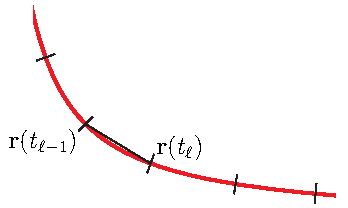
\includegraphics{parCurveL.pdf}
\end{center}
\end{nfig}


\item[$\circ$]
This gives us, as an approximate mass for $\cC$ of
\begin{equation*}
\sum_{\ell=1}^n \rho\big(\vr(t_\ell)\big)
    \big|\vr\big(t_\ell\big)-\vr\big(t_{\ell-1}\big)\big|
=\sum_{\ell=1}^n \rho\big(\vr(t_\ell)\big)
   \bigg|\frac{\vr\big(t_\ell\big)-\vr\big(t_{\ell-1}\big)}
                          {t_\ell-t_{\ell-1}}\bigg|\De t
\end{equation*}
\end{itemize}
Then we take the limit as $n\rightarrow\infty$. 
Assuming\footnote{We could
relax these conditions somewhat by instead assuming that $\vr'(t)$ 
and $\rho(t)$ are bounded and are continuous except at a finite number
of points. ($\vr'(t)$ need not exist at all at those points.)}
 that $\vr(t)$ is continuously differentiable and that $\rho(\vr)$ 
is continuous we get
\begin{equation*}
\text{Mass of $\cC$} = \int_a^b \rho\big(\vr(t)\big) \left|\diff{\vr}{t}(t)\right|\,\dee{t}
\end{equation*}
which we take to be a definition.
\begin{defn}\label{def:lineIntegral}
\begin{enumerate}[(a)]
\item
For a parametrized curve $\big(x(t),y(t), z(t)\big)$, $a\le t\le b$,
in $\bbbr^3$ that we call $\cC$, and for a function $f(x,y,z)$, we define
\begin{equation*}
\int_\cC f(x,y,z)\,\dee{s} 
 =\int_a^b f\big(x(t), y(t) , z(t) \big)\sqrt{x'(t)^2+y'(t)^2+z'(t)^2}\ 
       \dee{t}
\end{equation*}
In this notation the subscript $\cC$ specifies the curve, and $\dee{s}$
signifies arc length.

\item  
For a curve $y=f(x)$, $a\le x\le b$, in $\bbbr^2$ that we call $C$, 
and for a function $g(x,y)$, we define
\begin{equation*}
\int_C g(x,y)\,\dee{s} 
 =\int_a^b g\big(x, f(x) \big)\sqrt{1+f'(x)^2}\ 
       \dee{x}
\end{equation*}
\end{enumerate}
\end{defn}

\begin{eg}\label{eg:CofMass}
Suppose that we have a helical wire\footnote{For example, your favourite
solenoid or spring or slinky.}
\begin{equation*}
\vr(t) = \big(x(t)\,,\,y(t)\,,\,z(t)\big)
       =\big(a\cos t\,,\,a\sin t\,,\, bt\big)\qquad 0\le t\le 2\pi
\end{equation*}
and that this wire has constant mass density $\rho$.
Let's find the centre of mass of the wire. Recall that the centre of mass
is $\big(\bar x,\bar y,\bar z)$ with, for example, $\bar x$ being the
weighted average 
\begin{equation*}
\bar x = \frac{\int x\rho \dee{s}}{\int \rho\dee{s}}
= \frac{\int x \dee{s}}{\int \dee{s}}
\qquad\text{(since $\rho$ is constant)}
\end{equation*}
of $x$ over the wire. Similarly
$
\bar y = \frac{\int y \dee{s}}{\int \dee{s}}
$
and
$
\bar z = \frac{\int z \dee{s}}{\int \dee{s}}
$.
For the given curve
\begin{align*}
 \big(x(t)\,,\,y(t)\,,\,z(t)\big) &=\big(a\cos t\,,\,a\sin t\,,\, bt\big) \\
 \big(x'(t)\,,\,y'(t)\,,\,z'(t)\big) &=\big(-a\sin t\,,\,a\cos t\,,\, b\big) \\
\diff{s}{t}(t) &=\sqrt{x'(t)^2+y'(t)^2+z'(t)^2}
                  =\sqrt{a^2\sin^2t+a^2\cos^2t+b^2}
                  =\sqrt{a^2+b^2}
\end{align*}
so that
\begin{align*}
\bar x
&= \frac{\int x \dee{s}}{\int \dee{s}}
= \frac{\int_0^{2\pi} x(t) \sqrt{a^2+b^2}\,\dee{t}}
          {\int_0^{2\pi} \sqrt{a^2+b^2}\,\dee{t}}
= \frac{\int_0^{2\pi} a\cos(t) \,\dee{t}}{2\pi}
=0
\\
\bar y
&= \frac{\int y \dee{s}}{\int \dee{s}}
= \frac{\int_0^{2\pi} y(t) \sqrt{a^2+b^2}\,\dee{t}}
       {\int_0^{2\pi} \sqrt{a^2+b^2}\,\dee{t}}
= \frac{\int_0^{2\pi} a\sin(t) \,\dee{t}}{2\pi}
=0\\
\bar z
&= \frac{\int z \dee{s}}{\int \dee{s}}
= \frac{\int_0^{2\pi} z(t) \sqrt{a^2+b^2}\,\dee{t}}
      {\int_0^{2\pi} \sqrt{a^2+b^2}\,\dee{t}}
= \frac{\int_0^{2\pi} bt \,\dee{t}}{2\pi}
=\frac{b}{2\pi}\Big[\frac{t^2}{2}\Big]_0^{2\pi}
=b\pi
\end{align*}
So the centre of mass is right on the axis of the helix, half way up,
which makes perfect sense. 
\end{eg}


\section{Sliding on a Curve}\label{sec:Sliding}

We are going to investigate the motion of a particle of mass
$m$ sliding on a frictionless\footnote{We are mathematicians --- we like idealized situations.}, smooth curve that lies in a vertical
plane. We will consider three scenarios:
\begin{itemize}\itemsep1pt \parskip0pt \parsep0pt %\itemindent-15pt
\item[$\circ$] 
First, to set things up we'll look at a bead sliding on a stiff wire.
\item[$\circ$] 
Then, we will imagine that we are skiing straight
downhill and ask ``Where on the hill can we become airborne?".
\item[$\circ$] 
Then we will imagine that we are skateboarding in a 
culvert (a large pipe) and ask ``When is it safe?''.
\end{itemize}

\subsection*{The Sliding Bead}
First, consider a bead of mass $m$ that is sliding, without friction, 
on a stiff wire. According to Newton's law of motion
\begin{equation*}
m\va = \vF
\end{equation*}
where $\vF$ is the net force being applied to the bead. The bead is
subject to two forces. The gravitational force is $-mg\hj$. By
definition, absence of friction means that the wire is does not apply
any force that is in the direction tangential to the wire. But, because
it is stiff, the wire never changes shape and instead applies just the right 
amount of force, in the direction normal to the wire, that is needed 
to keep the bead on the wire\footnote{This force is required to keep 
the bead from either passing through the wire or flying off the wire.} 
without bending the wire. Call this normal force $W\hat\vN$.
\begin{efig}
\begin{center}
    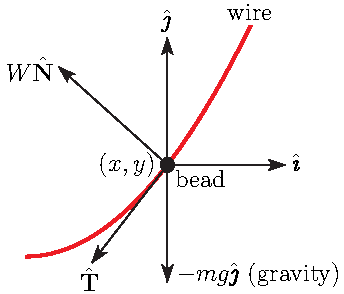
\includegraphics{wireC.pdf} 
\end{center}
\end{efig}
So, by Newton's law,
\begin{align*}\label{eq:normalComp}
m\,\va=-mg\,\hj+W\,\hat\vN
\end{align*}
We'll analyse this equation by splitting it into its tangential and
normal components.

To extract the tangential component of Newton's law, we dot it with 
$\vv=|\vv|\hat\vT$. Since $\hat\vT\cdot\hat\vN=0$ this kills all normal 
components.
\begin{align*}
m\vv\cdot\diff{\vv}{t}
&=-mg\hj\cdot\vv+W\hat\vN\cdot\vv\\
\frac{1}{2}m\diff{\ }{t}(\vv\cdot\vv)&=-mg\diff{y}{t}
\end{align*}
Here we have used 
\begin{itemize}\itemsep1pt \parskip0pt \parsep0pt %\itemindent-15pt
\item[$\circ$]
Theorem \ref{thm:DIFFalgebra}.c on the left hand side and
\item[$\circ$]
that $\hj\cdot\vv$ is just the $y$ component of $\vv$ and
\item[$\circ$]
that $\hat\vN$ and $\vv=|\vv|\hat\vT$ are perpendicular. 
\end{itemize}
Moving everything to the left hand side of the equation gives 
\begin{align*}
\diff{\ }{t}\left(\frac{1}{2}m|\vv|^2+mgy\right)&=0
\end{align*}
and we conclude that the quantity
\begin{impeqn}[Conservation of Energy]\label{eqn:consEnergy}
\begin{equation*}
E=\frac{1}{2}m|\vv|^2+mgy
\end{equation*}
\end{impeqn}\noindent
is a constant, independent of time. This is, of course, the 
principle of conservation of 
energy. It determines the speed $|\vv|=\sqrt{\frac{2E}{m}-2gy}$ of
the bead as a function of the height $y$ (and of the energy $E$, 
which is determined by the initial conditions).

To extract the normal component of Newton's law, 
we dot it with $\hat\vN$:
\begin{equation*}
m\va\cdot \hat\vN=-mg\hj\cdot \hat\vN+W
\end{equation*}
Since 
\begin{equation*}
\va=\difftwo{s}{t}\,\hat\vT+\ka\Big(\diff{s}{t}\Big)^2\hat\vN
=\difftwo{s}{t}\,\hat\vT+\ka|\vv|^2\hat\vN
\end{equation*}
and $\hat\vT$ and $\hat\vN$ are perpendicular, this gives, after a little
rearrangement,
\begin{impeqn}[Normal Force]\label{eqn:normalForce}
\begin{equation*}
W=m\ka|\vv|^2+mg\hj\cdot \hat\vN
=2\ka(E-mgy)+mg\hj\cdot \hat\vN
\end{equation*}
\end{impeqn}

\subsection*{The Skier}
The difference between the bead on the wire and the skier on
the hill is that while the hill is capable of applying an upward normal
force (i.e. it can push you upward to keep you from falling to 
the centre of the Earth), it is not capable of applying a downward 
normal force. That is the hill cannot pull down on you to keep you 
on the hill. Only gravity can keep you grounded. There are two 
main possibilities\footnote{We assume that you are going downhill and that the
curvature $\ka>0$.}.

\begin{efig}
\begin{center}
    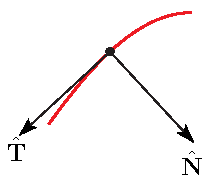
\includegraphics{wireD.pdf} \qquad\qquad
    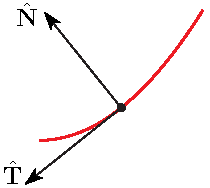
\includegraphics{wireU.pdf}
\end{center}
\end{efig}


\begin{itemize}\itemsep1pt \parskip0pt \parsep0pt %\itemindent-15pt
\item[$\circ$]
If the hill is concave downward as in the figure
on the left above, then $\hat\vN$ points downward and the hill is 
allowed to have
$W\le 0$ (which corresponds to the normal force $W\hat\vN$ pushing upward). 
If ever $W>0$, the hill would have to pull on you to keep you on hill. 
It can't, so you become airborne. Since $\hj\cdot \hat\vN<0$, this happens
whenever 
\begin{align*}
W>0 &\iff m\ka|\vv|^2+mg\hj\cdot \hat\vN >0 
    \iff |\vv| > \sqrt{\frac{g}{\ka}|\hj\cdot \hat\vN|}
\end{align*}

\item[$\circ$] 
If the hill is concave upward as in the figure
on the right above, then $\hat\vN$ points upward and the hill is 
allowed to have $W\ge 0$ (which corresponds to the normal force 
$W\hat\vN$ pushing upward). Since $\hj\cdot \hat\vN>0$ we always 
have $W=m\ka|\vv|^2+mg\hj\cdot \hat\vN > 0$.
You never become airborne. On the other hand your knees may complain.
\end{itemize}


\subsection*{The Skate Boarder}
So far, Equations \eqref{eqn:consEnergy} and \eqref{eqn:normalForce} 
apply to any stiff frictionless ``wire''. We now 
specialize  to the special case of a skateboarder inside a circular culvert 
of radius $a$. Let's put the bottom of the circle at the origin $(0,0)$,
so that the centre of the circle is at $(0,a)$.

\begin{efig}
\begin{center}
    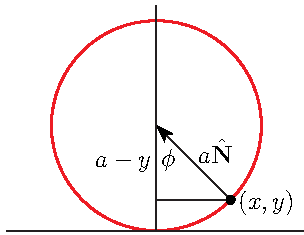
\includegraphics{circleC2.pdf}
\end{center}
\end{efig}
\noindent
In this case the curvature is $\ \ka=\frac{1}{a}\ $
and
$
\hj\cdot\hat\vN=\cos \phi=\frac{a-y}{a}
$
so \eqref{eqn:consEnergy} and \eqref{eqn:normalForce}  simplify to
\begin{align*}
|\vv|&=\sqrt{\frac{2}{m}(E-mgy)}=\sqrt{2g\Big(\frac{E}{mg}-y\Big)}
\\
W&=\frac{2}{a}(E-mgy)+\frac{mg}{a}(a-y)
=\frac{3mg}{a}\Big(\frac{2}{3mg}E+\frac{a}{3}-y\Big)
\end{align*}
Imagine now that you start at the bottom of the culvert, that is at $y=0$,
with energy $E>0$. As time progresses, $y$ increases and consequently $|\vv|$
and $W$ both decrease, as, of course, they should. This continues until one of the following three things happen.
\begin{enumerate}[(i)]
\item 
$|\vv|$ hits 0, in which case you stop rising and start descending. 
The speed $|\vv|$ is zero when $y=y_S=\frac{E}{mg}$.
(The subscript ``$S$'' stands for ``stop''.) Physicists say that 
when you reach $y_S$ all of your kinetic energy ($\frac{1}{2}m|\vv|^2$)
has been converted into potential energy ($mgy$). 

\item
$W$ hits zero. When you get higher than this, $W$ becomes negative 
and the culvert would have to pull on you to keep your feet on the culvert. 
As the culvert can only push on you, you become airborne. The normal force 
$W$ is zero  when $y=y_A=\frac{2}{3}\frac{E}{mg}+\frac{a}{3}$.
(The subscript ``$A$'' stands for ``airborne''.)

\item
$y$ hits $2a$. This is the summit of the culvert. You descend on the other side.
\end{enumerate}
Which case actually happens is determined by the relative sizes of $y_S,\ y_A$ and $2a$.
\begin{itemize}\itemsep1pt \parskip0pt \parsep0pt %\itemindent-15pt
\item[$\circ$]
Comparing 
$y_S=\frac{2}{3}\frac{E}{mg}+\frac{1}{3}\frac{E}{mg}$ and
$y_A=\frac{2}{3}\frac{E}{mg}+\frac{a}{3}$, we see that
$y_S\le y_A\iff \frac{E}{mg}\le a $.

\item[$\circ$] Comparing 
$y_A=\frac{2}{3}\frac{E}{mg}+\frac{a}{3}$ and
$a=\frac{2}{3}a+\frac{a}{3}$, we see that
$y_A\le a\iff \frac{E}{mg}\le a$.


\item[$\circ$] 
Comparing 
$y_A=\frac{2}{3}\frac{E}{mg}+\frac{a}{3}$ and
$2a=\frac{5}{3}a+\frac{a}{3}$, we see that
$y_A\le 2a\iff \frac{E}{mg}\le \frac{5}{2}a$.

\end{itemize}
So the conclusions are:
\begin{itemize}\itemsep5pt \parskip0pt \parsep0pt %\itemindent-15pt
\item[$\circ$]
{\bf If}  $\ {\bf 0\le\frac{E}{mg}\le a}\ $ then 
           $\ 0\le y_S\le y_A\le a\ $. 
In this case you just oscillate between heights 0 and $y_S\le a$ in 
the bottom half of the culvert, as in the figure on the left below.

\item[$\circ$]{
\bf If} $\ {\bf a\le\frac{E}{mg}\le \frac{5}{2}a}\ $ then 
$\ a\le y_A\le y_S,2a\ $.
In this case you make it more than half way to the top. But you 
become airborne at $y=y_A$ which is somewhere between the half way mark 
$y=a$ and the top $y=2a$. 
At this point our model breaks down because you are no longer in 
contact with the culvert. You just freely follow a parabolic arc until 
you crash back into the culvert, as in the figure in the centre below.

\item[$\circ$]
{\bf If} $\ {\bf \frac{5}{2}a < \frac{E}{mg}}\ $ then 
$\ 2a < y_A < y_S\ $.
In this case you
successfully go all the way around the culvert, looping  the loop,
as in the figure on the right below. Note that, as 
$\frac{E}{mg} > \frac{5}{2}a >2a$,  this requires significantly
more energy than that required to reach the top, i.e. to reach height $2a$.
\end{itemize}

\begin{efig}
\begin{center}
    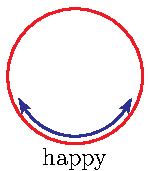
\includegraphics{skateA.pdf} \qquad\quad
    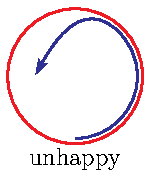
\includegraphics{skateB.pdf} \qquad\quad
    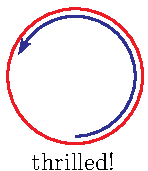
\includegraphics{skateC.pdf} 
\end{center}
\end{efig}

\section{Optional --- Polar Coordinates}\label{sec:polar}

So far we have always written vectors in two dimensions in terms of the basis vectors
$\hi$ and $\hj$. This is not always convenient. For example, when working in 
polar coordinates it is often convenient to use basis vectors
$\hat\vr(\theta)$, $\hat\vth(\theta)$ which depend on the value of the
current polar coordinate $\theta$ --- though one usually just writes 
$\hat\vr$, $\hat\vth$, suppressing the dependence on $\theta$ from 
the notation. When one is at the point with polar coordinates
$(r,\theta)$, these basis vectors are defined by
\begin{impeqn}\label{eqn:polarBasis}
\begin{align*}
\hat\vr(\theta) &= \cos\theta\,\hi + \sin\theta\,\hj \\
\hat\vth(\theta) &= -\sin\theta\,\hi + \cos\theta\,\hj \qquad\qquad
   \raisebox{-45pt}[15pt][40pt]{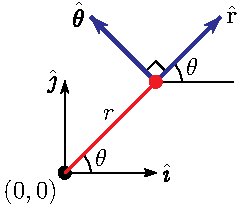
\includegraphics{polar.pdf}}
   \qquad\qquad\qquad
\end{align*}
\end{impeqn}\noindent
Note that this basis has two very nice properties.
\begin{enumerate}
\item
$|\hat\vr(\theta)| = |\hat\vth(\theta)| = 1$,\ \  
   $\hat\vr(\theta) \perp \hat\vth(\theta)$  (orthonormality)
\item
$\diff{\hat\vr}{\theta}(\theta)= \hat\vth(\theta)$,\ \  
$\diff{\hat\vth}{\theta}(\theta) = -\hat\vr(\theta)$
\end{enumerate}
That $\diff{\hat\vr}{\theta}(\theta)$ is some scalar multiple of 
$\hat\vth(\theta)$ follows just from the fact that $|\hat\vr(\theta)| = 1$.
\begin{align*}
|\hat\vr(\theta)| = 1 &\implies \hat\vr(\theta)\cdot\hat\vr(\theta)=1 \\
             &\implies \hat\vr(\theta)\cdot \diff{\hat\vr}{\theta}(\theta)
                                =\frac{1}{2}\diff{\hfill}{t}\big(
                                   \hat\vr(\theta)\cdot\hat\vr(\theta)\big)
                                =0 \\
         &\implies  \diff{\hat\vr}{\theta}(\theta)\perp \hat\vr(\theta)
         \implies \diff{\hat\vr}{\theta}(\theta)\parallel \hat\vth(\theta)
\end{align*}
Similarly, that $\diff{\hat\vth}{\theta}(\theta)$ is some scalar 
multiple of $\hat\vr(\theta)$ follows just from the fact 
that $|\hat\vth(\theta)| = 1$.

\begin{lemma}\label{lem:polar}
If we parametrize a curve by giving its polar coordinates\footnote{As usual $r$ is the distance from the origin to the point and $\theta$ is angle between the $x$-axis and the vector from the origin to the point. The symbols $r$, $\theta$
are the standard mathematics symbols for the polar coordinates. Appendix \ref{ap:ISO} gives another set of symbols that is commonly used in the physical sciences and engineering.} $\big(r(t)\,,\,\theta(t)\big)$, then
\begin{enumerate}[(a)]
\item
\  $\vr(t) = r(t)\ \hat\vr\big(\theta(t)\big)$
\item
\  $\vv(t) = \diff{r}{t}(t)\ \hat\vr\big(\theta(t)\big) 
             + r(t)\ \diff{\theta}{t}(t)\ \hat\vth\big(\theta(t)\big)$
\item
\  $\va(t) = 
\Big(\difftwo{r}{t}(t)-r(t)\big(\diff{\theta}{t}(t)\big)^2\Big) 
             \hat\vr\big(\theta(t)\big)
   +\Big(r(t)\ \difftwo{\theta}{t}(t) 
          + 2 \diff{r}{t}(t)\diff{\theta}{t}(t)\Big)
                  \hat\vth\big(\theta(t)\big)$
\end{enumerate}
\end{lemma}
\noindent It is standard to suppress the arguments $t$ and $\theta(t)$
and write, for example,
\begin{equation*}
\vv= \diff{r}{t}\ \hat\vr
             + r\ \diff{\theta}{t}\ \hat\vth
\end{equation*}
But it is important to remember that the arguments really are there.
\begin{proof}

The vector from the origin to the point whose 
polar coordinates are 
$(r,\theta)$ is $\vr = r\,\hat\vr(\theta)$. So if we parametrize a curve by 
giving the polar coordinates at time $t$,
\begin{align*}
\vr(t) &= r(t)\ \hat\vr\big(\theta(t)\big)
 \\
\vv(t) &= \diff{r}{t}(t)\ \hat\vr\big(\theta(t)\big) +
              r(t)\ \diff{\hat\vr}{\theta}\big(\theta(t)\big)\ 
              \diff{\theta}{t}(t) \notag\\
        &= \diff{r}{t}(t)\ \hat\vr\big(\theta(t)\big) 
             + r(t)\ \diff{\theta}{t}(t)\ \hat\vth\big(\theta(t)\big)
\\
%        &= \diff{r}{t}\ \hat\vr 
%             + r\ \diff{\theta}{t}\ \hat\vth \\
\va(t) & = \difftwo{r}{t}\ \hat\vr 
                + \diff{r}{t}\ \diff{\hat\vr}{\theta}\ \diff{\theta}{t} 
             + \diff{r}{t}\ \diff{\theta}{t}\ \hat\vth
             + r\ \difftwo{\theta}{t}\ \hat\vth
             + r\ \Big(\diff{\theta}{t}\Big)^2\ \diff{\hat\vth}{\theta} 
\\
       &=\Big(\difftwo{r}{t}-r\ \Big(\diff{\theta}{t}\Big)^2\Big) \hat\vr
   +\Big(r\ \difftwo{\theta}{t} + 2 \diff{r}{t}\ \diff{\theta}{t}\Big)\hat\vth
\end{align*}
\end{proof}

\begin{eg}\label{eg:beadToss}
As an example, consider a bead that is sliding on a frictionless rod
that has one end fixed at the origin and that is rotating about the
origin at a constant $\Omega\,$rad/sec. 
\begin{efig}
\begin{center}
    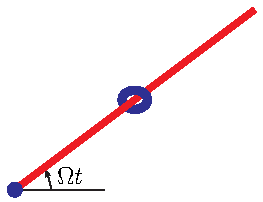
\includegraphics{beadRod.pdf}
\end{center}
\end{efig}
Because the rod is frictionless, 
it is incapable of applying to the bead any force parallel to the rod. So 
under Newton's law, $m\va=\vF$, the radial\footnote{The $\hat\vth$ component
of the acceleration just tells us how much normal force the rod is applying
to the bead to keep it on the rod.} component of the acceleration
of the particle is exactly zero. So, if the polar coordinates of the bead
at time $t$ are $\big(r(t),\theta(t)\big)$, then,
by Lemma \ref{lem:polar}.c,
\begin{equation*}
\difftwo{r}{t}-r\ \Big(\diff{\theta}{t}\Big)^2 = 0
\end{equation*}
As the rod is rotating at $\Omega\,$rad/sec,
$\diff{\theta}{t}=\Omega$ and
\begin{equation*}
\difftwo{r}{t}-\Omega^2\ r = 0
\end{equation*}
The general solution to this constant coefficient second order
ordinary differential equation is\footnote{A review of the technique used to find this solution is given in Appendix \ref{ap:ODE}. In any event, it is easy to check that $r(t)=A e^{\Omega\,t} + B e^{-\Omega\,t}$ really does obey
$\difftwo{r}{t}-\Omega^2\ r = 0$.} 
$$
r(t)  = A e^{\Omega\,t} + B e^{-\Omega\,t}
$$ 
where $A$ and $B$ are arbitrary constants that are determined by initial
conditions. 
Just as an example, if $r(0)= 1$ and $r'(0)= 0$,
then $A+B=1$ and $A\Omega-B\Omega=0$, so that $A=B=\frac{1}{2}$ and
\begin{equation*}
r(t)  = \frac{1}{2}\big(e^{\Omega\,t}+e^{-\Omega\,t}\big)\qquad
\end{equation*}
If, again for example, $\theta(0) = 0$, then $\theta(t) = \Omega t$
and the bead follows the polar coordinate curve
\begin{equation*}
r(\theta) = \frac{1}{2}\big(e^{\theta}+e^{-\theta}\big)
\end{equation*}
Observe that $r(\theta)$ is $1$ when $\theta=0$, increases as $\theta$ increases, and tends to $\infty$ as $\theta\rightarrow+\infty$. The curve is a spiral.
\begin{efig}
\begin{center}
    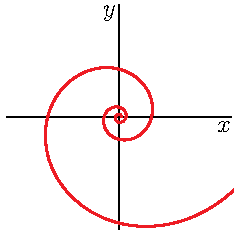
\includegraphics{beadCurve.pdf}
\end{center}
\end{efig}
\end{eg}

\begin{eg}[Conic sections in polar coordinates]\label{eg:conicA}
In this example, we derive the equation of a general conic section in 
polar coordinates. A conic section is the intersection of a plane with a cone.
This is illustrated in the figures below.
\vadjust{
\begin{efig}
\begin{center}
    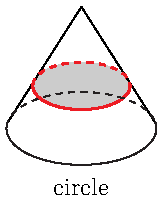
\includegraphics{conePlaneCircle.pdf}\quad
    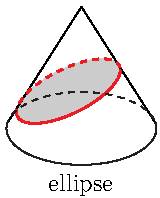
\includegraphics{conePlaneEllipse.pdf}\quad
    \includegraphics{conePlaneParabola.pdf}\quad
    \includegraphics{conePlaneHyperbola.pdf}
\end{center}
\end{efig}
}
For our current purposes, it is convenient to use the 
equivalent\footnote{It is outside our scope to prove this equivalence.} 
(and often used) definition that a conic section is the set of points $P$ 
in the $xy$-plane 
\begin{itemize}\itemsep1pt \parskip0pt \parsep0pt %\itemindent-15pt
\item
whose distance from a fixed point $F$ (called the \emph{focus} of the conic) 
\item
is a constant multiple $\veps\ge 0$ (called the \emph{eccentricity} 
of the conic)
\item  
of the distance from $P$ to a fixed line $L$ (called the \emph{directrix} 
of the conic).
\end{itemize}
Choose a coordinate system with the focus $F$ of the conic being the origin
and with the directrix $L$ being $x=p$ for some $p>0$. 
\begin{efig}
\begin{center}
    \includegraphics{conic.pdf}
\end{center}
\end{efig}
If $P$ has polar coordinates $(r,\theta)$, then $P$ has $x$-coordinate
$r\cos\theta$. The point $Q$ on the line $L$ in the figure above 
has $x$-coordinate $p$.
So the distance from $P$ to $L$, which is also the distance from $P$ to
$Q$, is $p-r\cos\theta$.  The distance from $P$ to $F$ is $r$. We require that 
the distance from $P$ to $F$ is $\veps$ times the distance from $P$ to $L$.
So
\begin{equation*}
r=\veps\big(p-r\cos\theta\big)
\iff 
r=\frac{\veps p}{1+\veps\cos\theta}
\end{equation*}
The numerator $\veps p$ is usually renamed to $\ell$ giving the equation
\begin{equation*}
r=\frac{\ell}{1+\veps\cos\theta}
\end{equation*}
\end{eg}


\begin{eg}[Conic sections in polar coordinates, again]\label{conicB}
We'll now take the equation $r=\frac{\ell}{1+\veps\cos\theta}$
for a conic section in polar coordinates, from the last example, 
and convert it to the more familiar Cartesian coordinates. Just by the 
definition of polar coordinates
\begin{align}
r\big(1+\veps\cos\theta\big)=\ell
&\iff r = \ell -\veps x \notag\\
&\iff x^2+y^2 = \ell^2-2\veps\ell x+\veps^2 x^2  \notag\\
&\iff (1-\veps^2) x^2  + 2\veps\ell x + y^2 = \ell^2
\tag{C}%\label{eqn:conicCartA}
\end{align}
Now consider separately four different cases, depending on the value of 
$\veps \ge 0$.
\begin{itemize}
\item 
If $\veps=0$, (C) reduces to 
\begin{equation*}
x^2+y^2 = \ell^2\qquad\qquad
   \raisebox{-35pt}[20pt][25pt]{\includegraphics{conicCircle.pdf}}
\end{equation*}
which is of course a circle of radius $\ell$.

\item 
If $0<\veps<1$, completing the square in (C) 
gives
\begin{equation*}
(1-\veps^2)\Big(x+\frac{\veps\ell}{1-\veps^2}\Big)^2 + y^2
   = \ell^2 + \frac{\veps^2\ell^2}{1-\veps^2}
   =  \frac{\ell^2}{1-\veps^2}
\end{equation*}
which is equivalent to
\begin{equation*}
\frac{\big(x+\frac{\veps\ell}{1-\veps^2}\big)^2}
              { \frac{\ell^2}{{(1-\veps^2)}^2}}
+\frac{y^2}{\frac{\ell^2}{1-\veps^2}}
=1
 \qquad\quad  \raisebox{-35pt}[15pt][28pt]{\includegraphics{conicEllipse.pdf}}
\end{equation*}
and is of course an ellipse with semi-major axis $r_M=\frac{\ell}{1-\veps^2}$
and semi-minor axis $r_m=\frac{\ell}{\sqrt{1-\veps^2}}$.

\item 
If $\veps=1$, (C) reduces to 
\begin{equation*}
y^2 = \ell^2-2\ell x
 \qquad\qquad  \raisebox{-40pt}[15pt][20pt]{\includegraphics{conicParabola.pdf}}
\end{equation*}
which is of course a parabola.

\item
If $\veps>1$, the same computation as in the $0<\veps<1$ case 
gives
\begin{equation*}
\frac{\big(x-\frac{\veps\ell}{\veps^2-1}\big)^2}
              { \frac{\ell^2}{{(\veps^2-1)}^2}}
-\frac{y^2}{\frac{\ell^2}{\veps^2-1}}
=1
 \qquad\quad  \raisebox{-50pt}[30pt][28pt]{\includegraphics{conicHyperbola.pdf}}
\end{equation*}
and is of course a hyperbola.
\end{itemize}
\end{eg}


\section{Optional --- Central Forces}\label{sec:central forces}

One of the great triumphs of Newtonian mechanics was the explanation
of Kepler's laws\footnote{The German astronomer Johannes Kepler (1571--1630) 
developed these laws during the course of an attempt to relate the five extraterrestrial planets then known to the five Platonic solids. He based
the laws on a great number of careful measurements 
made by the Danish Astronomer Tycho Brahe (1546--1601). Then
Isaac Newton (English, 1642--1727) provided the explanation in 1687.
Kepler also wrote a paper entitled ``On the Six-Cornered Snowflake''.
Tycho Brahe lost his nose in a sword duel and wore a prosthetic nose
from then on. 
%The story is that Brahe died of pneumonia
%contracted when, after a night of drinking with the Danish king, the king
%fell into a canal and Brahe jumped in after him.
The story is that Brahe died from a burst bladder that resulted 
from his refusing to leave the dinner table before his host.}, 
which said
\begin{enumerate}\itemsep1pt \parskip0pt \parsep0pt %\itemindent-15pt
\item 
The planets trace out ellipses about the sun as focus.
\item
The radius vector $\vr$ sweeps out equal areas in equal times. 
\item
The square of the period of each planet is proportional to the cube of the major axis of the planet's orbit.
\end{enumerate}
Newton showed that all of these behaviours follow from the assumption
that the acceleration $\va(t)$ of each planet  obeys the law of
motion $m\va =\vF$ where $m$ is the mass of the planet and 
\begin{equation*}
\vF = -\frac{GMm}{r^3}\vr
\end{equation*}
is the ``gravitational force'' applied on the planet by the sun. Here
$G$ is a constant\footnote{Its value is about $6.67408\times10^{-11} \text{m}^3\,\text{kg}^{-1}\,\text{sec}^{-2}$.}, 
called the ``gravitational constant'' or the
``universal gravitational constant'', $M$ is the mass of the 
sun, $\vr$ is the vector from the sun to the planet and $r=|\vr|$. 

In this section, we'll show that some of these properties follow from the
weaker assumption that the acceleration $\va(t)$ of each planet 
obeys the law of motion $m\va =\vF$ with $\vF$ being a central force.
That is, the assumption that $\vF$ is parallel to $\vr$. The verification that 
the other properties follow from the specific form of the gravitational 
force, proportional to $r^{-2}$, will be delayed until the 
optional \S\ref{sec:planet}. 

So, in this section, we assume that we have a parametrized
curve $\vr(t)$ and that this curve obeys
\begin{equation*}
m\difftwo{\vr}{t}(t) = \vF\big(\vr(t)\big)
\end{equation*}
where, for all $\vr\in\bbbr^3$, $\vF(\vr)$ is parallel to $\vr$. We shall show that
\begin{enumerate}\itemsep1pt \parskip0pt \parsep0pt %\itemindent-15pt
\item 
The path $\vr(t)$ lies in a plane through the origin and that
\item
the radius vector $\vr$ sweeps out equal areas in equal times. 
\end{enumerate}
We'll start by trying to guess what the plane is. Pretend that we know that 
$\vr(t)$ lies in a fixed plane through the origin. Then 
$\vv(t)=\diff{\vr}{t}(t)$ lies in the same plane and 
$\vr(t)\times\vv(t)$ is perpendicular to the plane. If our path really does
lie in a fixed plane, $\vr(t)\times\vv(t)$ cannot change direction --- it must 
always be parallel to the normal vector to the plane. So let's define
\begin{equation*}
\vOm(t) = \vr(t)\times\vv(t)
\end{equation*}
and check how it depends on time. By the product rule,
\begin{equation}
\diff{\vOm}{t}(t) =\diff{\ }{t}\big(\vr(t)\times\vv(t)\big)
=\vv(t)\times\vv(t) + \vr(t)\times\va(t)
=\frac{1}{m}\vr(t)\times\vF\big(\vr(t)\big)
=\vZero
\tag{A}\end{equation}
because $\vr(t)$ and $\vF\big(\vr(t)\big)$ are parallel.
So $\vOm(t)$ is\footnote{Physicists call $m\,\vOm(t)$ the angular momentum at time $t$ and refer to (A) as (an example of) conservation of angular momentum.
Conservation of angular momentum is exploited in gyro-compasses and by 
ice skaters (to spin faster/slower).} 
in fact independent of $t$. It is a constant vector that
we'll just denote $\vOm$. 

As $\vr(t)\times\vv(t)=\vOm$, we have that
$\vr(t)$ is always perpendicular to $\vOm$ and
\begin{equation*}
\vr(t)\cdot\vOm =0
\end{equation*}
\begin{itemize}\itemsep1pt \parskip0pt \parsep0pt %\itemindent-15pt
\item[$\circ$]
If $\vOm\ne \vZero$, this is exactly the statement that $\vr(t)$ always 
lies in the plane through the origin with normal vector $\vOm$.
\item[$\circ$]
If $\vOm=\vZero$, then $\vr(t)$ is always parallel to $\vv(t)$ and there
is some function $\alpha(t)$ such that
\begin{equation*}
\diff{\vr}{t}(t) = \vv(t) = \alpha(t)\,\vr(t)
\end{equation*}
This is a first order, linear, ordinary differential equation that we can solve
by using an integrating factor. Set
\begin{equation*}
\beta(t) = \int_0^t\alpha(t)\ \dee{t}
\end{equation*}
Then
\begin{align*}
\diff{\vr}{t}(t) = \alpha(t)\,\vr(t)
&\iff e^{-\beta(t)} \diff{\vr}{t}(t) -\alpha(t)e^{-\beta(t)}\,\vr(t)=0\\
&\iff \diff{\ }{t}\big[e^{-\beta(t)}\vr(t)\big] = 0\\
&\iff e^{-\beta(t)}\vr(t) = \vr(0)\\
&\iff \vr(t) =  e^{\beta(t)}\vr(0)
\end{align*}
so that $\vr(t)$ lies on a line through the origin. This makes sense ---
the particle is always moving parallel to its radius vector.
\end{itemize}
This completes the verification that $\vr(t)$ lies in a plane through 
the origin.

Now we show that the radius vector $\vr(t)$ sweeps out equal areas in 
equal times. In other words, we now verify that the rate at which 
$\vr(t)$ sweeps out area is independent of time. To do so we rewrite the
statement that $|\vr(t)\times\vv(t)\big|$ is constant in polar coordinates.
Writing $\vr(t) = r(t)\hat\vr\big(\theta(t)\big)$ and then applying
Lemma \ref{lem:polar}.b gives that
\begin{align*}
\text{constant} = \big|\vr\times\vv\big| 
   = \Big|r\hat\vr\times\Big(\diff{r}{t}\ \hat\vr 
             + r\ \diff{\theta}{t}\ \hat\vth\Big)\Big|
   =r^2\diff{\theta}{t}
\qquad\text{since}\quad |\hat\vr\times\hat\vr|=0,\ 
                        |\hat\vr\times\hat\vth|=1
\end{align*}
is constant. It now suffices to observe that $r(t)^2\diff{\theta}{t}(t)$ 
is exactly twice the rate at which $\vr(t)$ sweeps out area. To see this,
just look at the figure below. The shaded area is essentially a wedge of
a circular disk of radius $r$. (If $r(t)$ were independent of $t$, it would be exactly a wedge of a circular disk.) Its area is the 
fraction $\frac{\dee{\theta}}{2\pi}$ of the area of the full disk, which is
\begin{equation*}
\frac{\dee{\theta}}{2\pi}\ \pi r^2 = \frac{1}{2}r^2\,\dee{\theta}
\qquad\qquad\raisebox{-0.35\height}[42pt][20pt]{\includegraphics{equalArea.pdf}}
\end{equation*}
  

\section{Optional --- Planetary Motion}\label{sec:planet}
We now return to the claim, made in \S\ref{sec:central forces} on central 
forces, that if $\vr(t)$ obeys Newton's inverse square law 
\begin{equation*}
\difftwo{\vr}{t} = -\frac{GM}{r^3}\vr = -\frac{GM}{r^2}\hat\vr
\end{equation*}
then the curve obeys Kepler's laws
\begin{enumerate}\itemsep1pt \parskip0pt \parsep0pt %\itemindent-15pt
\item 
$\vr(t)$ runs over an ellipse having one focus at the origin and
\item
$\vr(t)$ sweeps out equal areas in equal times and
\item
the square of the period is proportional to the cube of the major axis of the 
ellipse.
\end{enumerate}
We just showed, in \S\ref{sec:central forces}, that the fact that 
$-\frac{GM}{r^3}\vr$ is parallel to $\vr$ implies that $\vr(t)$
lies in a plane through the origin and sweeps out equal area in equal times.
We now verify the remaining Kepler laws.

We start by just rewriting Newton's laws above in polar coordinates.
We saw in Lemma \ref{lem:polar}.c, that if we write $\vr(t) = r(t)\,\hat\vr(t)$,
then 
\begin{align*}
\difftwo{\vr}{t} = 
  \left(\difftwo{r}{t}-r\ \left(\diff{\theta}{t}\right)^2\right) \hat\vr
  +\left(r\ \difftwo{\theta}{t} + 2 \diff{r}{t}\ \diff{\theta}{t}\right)\hat\vth
= -\frac{GM}{r^3}\vr
= -\frac{GM}{r^2}\hat\vr
\end{align*}
The $\hat\vr$ and $\hat\vth$ components of this equation are
\begin{align*}
\difftwo{r}{t}-r\ \left(\diff{\theta}{t}\right)^2 &= -\frac{GM}{r^2} \\[0.05in]
r\ \difftwo{\theta}{t} + 2 \diff{r}{t}\ \diff{\theta}{t} &= 0
\end{align*}
The second of these two equations only tells us that
\begin{equation*}
\diff{\ }{t}\left\{r^2\,\diff{\theta}{t}\right\} 
= r\left\{
     r\ \difftwo{\theta}{t} + 2 \diff{r}{t}\ \diff{\theta}{t}\right\} = 0
\implies 
r^2\,\diff{\theta}{t} = h,\quad\text{a constant}
\end{equation*}
which we already knew. Substituting $\diff{\theta}{t} =\frac{h}{r^2}$
into the first equation gives
\begin{equation}\label{eqn:planetRadialR}
\difftwo{r}{t}-\frac{h^2}{r^3} = -\frac{GM}{r^2} 
\end{equation}
This equations contains a lot of $\frac{1}{r}$'s. So let's set $u=\frac{1}{r}$.
Furthermore, for the first of Kepler's laws, we really want $r$ as a function of
$\theta$ rather than $t$. So let's make $u$ a function of $\theta$ and write
\begin{equation*}
r(t) = \frac{1}{u(\theta(t))}
\end{equation*}
Then
\begin{align*}
\diff{r}{t}(t) &= -\frac{1}{u^2}
        \diff{u}{\theta}\big(\theta(t)\big)\diff{\theta}{t}(t)
   = - h\diff{u}{\theta}\big(\theta(t)\big)\qquad
\text{since $\diff{\theta}{t} = \frac{h}{r^2}=hu^2$} \\
\difftwo{r}{t}(t) 
   &= -h\difftwo{u}{\theta}\big(\theta(t)\big)\diff{\theta}{t}(t)
     = -h^2 u\big(\theta(t)\big)^2 \difftwo{u}{\theta}\big(\theta(t)\big)
\end{align*}
and our equation becomes
\begin{equation}\label{eqn:planetRadialU}
-h^2u^2\difftwo{u}{\theta} -h^2u^3= -GM u^2\qquad\text{or}\qquad
\difftwo{u}{\theta} + u = \frac{GM}{h^2}
\end{equation}
This is a second order, linear, ordinary differential equation
with constant coefficients.  Recall\footnote{See Appendix \ref{ap:ODE}.} 
that the general solution of such an 
equation is the sum of a ``particular solution'' (i.e. any one solution,
which in this case we can take to be the constant function $\frac{GM}{h^2}$)
plus the general solution of the homogeneous equation
$u''+u=0$, which one often writes as
\begin{equation*}
A\cos\theta +B\sin\theta
\end{equation*}
with $A$ and $B$  arbitrary constants. In this particular application it is 
more convenient to write the solution in a different, standard but less
commonly used, form. Namely, we can use the triangle
\begin{efig}
\begin{center}
     \includegraphics{trianglePl.pdf}
\end{center}
\end{efig}
to write $A= C\cos\alpha$ and $B=C\sin\alpha$ so that 
the general solution of the homogeneous equation $u''+u=0$ becomes
\begin{equation*}
C\cos\alpha\cos\theta +C\sin\alpha\sin\theta
=C\cos(\theta-\alpha)
\end{equation*}
with $C$ and $\alpha$ being arbitrary constants. So the general solution 
to \eqref{eqn:planetRadialU} is
\begin{equation*}
u(\theta) = \frac{GM}{h^2} + C\cos(\theta-\alpha)
\end{equation*}
and the general solution to \eqref{eqn:planetRadialR} is
\begin{equation*}
r(t) = \frac{1}{\frac{GM}{h^2} + C\cos(\theta(t)-\alpha)}
\end{equation*}
The angle $\alpha$ just shifts the zero point of our coordinate $\theta$.
By rotating our coordinate system by $\alpha$, we can arrange that $\alpha=0$
and then
\begin{equation*}
r(t) = \frac{1}{\frac{GM}{h^2} + C\cos(\theta(t))}
     = \frac{\ell}{1+\veps\cos\theta}
\qquad\text{with}\quad
\ell=\frac{h^2}{GM},\ 
\veps=\frac{Ch^2}{GM}
\end{equation*}
As we saw in Example \ref{eg:conicA}, this is exactly the equation 
of a conic section with eccentricity $\veps$.

That leaves only the last of Kepler's laws, relating the period 
to the semi-major axis. As we are talking about planets, whose orbits 
remain bounded, our conic section must be a circle or ellipse, rather 
than a parabola or hyperbola.
Looking back at Example \ref{conicB}, we see that the semi-major 
and semi-minor axes of our ellipse are
\begin{align*}
a=\frac{\ell}{1-\veps^2}
\qquad
b=\frac{\ell}{\sqrt{1-\veps^2}}
\end{align*}
The period $T$ of our orbit is just the length of time it takes
the radius vector $\vr(t)$ to sweep out the area of the ellipse\footnote{You 
probably computed the area of an ellipse in first year calculus. If not,
you should be able to do it now in a few lines.},
which is $\pi ab$.  As the rate at which the radius vector is sweeping out 
area is $\frac{1}{2} r^2\diff{\theta}{t} = \frac{h}{2}$, we have
\begin{align*}
T^2 = \Big(\frac{\pi a b}{h/2}\Big)^2
    =\frac{4\pi^2 a^2 b^2}{h^2}
    =\frac{4\pi^2 a^2 b^2}{GM\ell}
    =\frac{4\pi^2}{GM}\ a^3\qquad
\text{since }\ell=\frac{b^2}{a}
\end{align*}



%\vfill\pagebreak

\section{Optional --- The Astroid}\label{sec:astroid}
Imagine a ball of radius $a/4$ rolling around the inside of a circle of
radius $a$. The curve traced by a point $P$ painted on the inner circle
(that's the blue curve in the figures below)
is called an astroid\footnote{The name ``astroid'' comes from the Greek word ``aster'', 
meaning star, with the suffix ``oid'' meaning ``having the shape of''. The curve was 
first discussed by Johann  Bernoulli in 1691--92.}.
We shall find its equation.
\begin{wfig}
\begin{center}
     \includegraphics{astroid1AA.pdf}\quad
     \includegraphics{astroid1BB.pdf}\quad
     \includegraphics{astroid1CC.pdf}
\end{center}
\begin{center}
     \includegraphics{astroid1DD.pdf}\quad
     \includegraphics{astroid1EE.pdf}\quad
     \includegraphics{astroid1FF.pdf}
\end{center}
\end{wfig}
Define the angles $\theta$ and $\phi$ as
in the figure in the left below.
\begin{wfig}
\begin{center}
     \includegraphics{astroid.pdf}\qquad\qquad
     \includegraphics{astroid3.pdf}
\end{center}
\end{wfig}
\noindent That is 
\begin{itemize}\itemsep1pt \parskip0pt \parsep0pt %\itemindent-15pt
\item[$\circ$]
the vector from the centre, $O$, of the circle of radius
$a$ to the centre, $Q$, of the ball of radius $a/4$ is
$
\frac{3}{4}a\big(\cos\theta,\sin\theta\big)
$
and
\item[$\circ$] the vector from the centre, $Q$, of the ball of radius $a/4$ to
the point $P$ is
$
\frac{1}{4}a\big(\cos\phi,-\sin\phi\big)
$
\end{itemize}
As $\theta$ runs from 0 to $\frac{\pi}{2}$, the point of contact
between the two circles travels through one quarter of the circumference
of the circle of radius $a$, which is a distance $\frac{1}{4}(2\pi a)$, 
which, in turn, is exactly the circumference of the inner circle. 
Hence if $\phi=0$ for $\theta=0$ (i.e. if $P$ starts on the $x$-axis), 
then for $\theta=\frac{\pi}{2}$, $P$ is back in contact with the big 
circle at the north pole of both the inner and outer circles. 
That is, $\phi=\frac{3\pi}{2}$ when $\theta=\frac{\pi}{2}$. 
(See the figure on the right above.) 
So $\phi=3\theta$  and $P$ has coordinates
\begin{equation*}
\frac{3}{4}a\big(\cos\theta,\sin\theta\big)
+\frac{1}{4}a\big(\cos\phi,-\sin\phi\big)
=\frac{a}{4}\big(3\cos\theta+\cos 3\theta,3\sin\theta-\sin 3\theta\big)
\end{equation*}
As, recalling your double angle, or even better your triple angle, 
trig identities,
\begin{align*}
\cos3\theta&=\cos\theta\cos2\theta-\sin\theta\sin 2\theta\\
&=\cos\theta[\cos^2\theta-\sin^2\theta]-2\sin^2\theta\cos\theta\\
&=\cos\theta[\cos^2\theta-3\sin^2\theta]\\
\sin3\theta&=\sin\theta\cos2\theta+\cos\theta\sin 2\theta\\
&=\sin\theta[\cos^2\theta-\sin^2\theta]+2\sin\theta\cos^2\theta\\
&=\sin\theta[3\cos^2\theta-\sin^2\theta]
\end{align*}
we have
\begin{equation*}
\begin{alignedat}{3}
3\cos\theta+\cos 3\theta
   &=\cos\theta[3+\cos^2\theta-3\sin^2\theta] &
   &=\cos\theta[3+\cos^2\theta-3(1-\cos^2\theta)] &
   &=4\cos^3\theta\\
3\sin\theta-\sin 3\theta
   &=\sin\theta[3-3\cos^2\theta+\sin^2\theta] &
   &=\sin\theta[3-3(1-\sin^2\theta)+\sin^2\theta] &
   &=4\sin^3\theta
\end{alignedat}
\end{equation*}
and the coordinates of $P$ simplify to
\begin{equation*}
x(\theta)= a\cos^3\theta\qquad y(\theta)=a\sin^3\theta
\end{equation*}
Oof! As
$\ 
x^{2/3}+y^{2/3}=a^{2/3}\cos^2\theta+a^{2/3}\sin^2\theta 
\ ,$
the path traced by $P$ obeys the equation
\begin{equation*}
x^{2/3}+y^{2/3} =a^{2/3}
\end{equation*}
which is surprisingly simple, considering what we went through to get here.

There remains the danger that there could exist points $(x,y)$ obeying
 the equation $x^{2/3}+y^{2/3}=a^{2/3}$ that are not of the form
$x= a\cos^3\theta,\ y=a\sin^3\theta$ for any $\theta$. That is, there is a danger
that the parametrized curve $x= a\cos^3\theta,\ y=a\sin^3\theta$ covers only
a portion of $x^{2/3}+y^{2/3}=a^{2/3}$. We now show that 
the parametrized curve $x= a\cos^3\theta,\ y=a\sin^3\theta$ in fact covers all
of $x^{2/3}+y^{2/3}=a^{2/3}$ as $\theta$ runs from $0$ to $2\pi$.

First, observe that $x^{2/3}=\big(\root 3\of x\big)^2\ge 0$ and 
$y^{2/3}=\big(\root 3\of y\big)^2\ge 0$. Hence, if $(x,y)$ obeys
$x^{2/3}+y^{2/3}=a^{2/3}$, then necessarily $0\le x^{2/3}\le a^{2/3} $
and so $-a\le x\le a$. As $\theta$ runs from $0$ to $2\pi$, $a\cos^3\theta$
takes all values between $-a$ and $a$ and hence takes all possible values
of $x$. For each $x\in[-a,a]$, $y$ takes two values, namely $\pm{[a^{2/3}-x^{2/3}]}^{3/2}$.
If $x=a\cos^3\theta_0=a\cos^3(2\pi-\theta_0)$, the two corresponding values 
of $y$ are precisely
$a\sin^3\theta_0$ and $-a\sin^3\theta_0=a\sin^3(2\pi-\theta_0)$.

\section{Optional --- Parametrizing Circles}\label{sec:paramCircles}
We now discuss a simple strategy for parametrizing circles in three
dimensions, starting with the circle in the $xy$-plane that has radius $\rho$
and is centred on the origin. This is easy to parametrize:
\begin{equation*}
\raisebox{-40pt}[70pt][40pt]{\smash{\includegraphics{circle1.pdf}}}\qquad\quad
\vr(t)=\rho\cos t\,\hi+ \rho\sin t\,\hj
\qquad 0\le t< 2\pi
\end{equation*}
Now let's move the circle so that its centre is at some general point
$\vc$. To parametrize this new circle, which still has radius $\rho$ and which 
is still parallel to the $xy$-plane, we just translate by $\vc$:
\begin{equation*}
\raisebox{-60pt}[60pt][58pt]{\smash{\includegraphics{circle2.pdf}}}\qquad\quad
\vr(t)=\vc+\rho\cos t\,\hi+ \rho\sin t\,\hj
\qquad 0\le t< 2\pi
\end{equation*}
Finally, let's consider a circle in general position. The secret to 
parametrizing a general circle is to replace $\hi$ and $\hj$ by two new vectors
$\hi'$ and $\hj'$ which 
\begin{enumerate}[(a)]\itemsep1pt \parskip0pt \parsep0pt %\itemindent-15pt
\item are unit vectors, 
\item are parallel to the plane of the desired circle and 
\item are mutually perpendicular.
\end{enumerate}
\begin{equation*}
\raisebox{-70pt}[50pt][70pt]{\smash{\includegraphics{circle3.pdf}}}\qquad\quad
\vr(t)=\vc+\rho\cos t\,\hi'+ \rho\sin t\,\hj'
\qquad 0\le t< 2\pi
\end{equation*} 
To check that this is correct, observe that
\begin{itemize}\itemsep1pt \parskip0pt \parsep0pt %\itemindent-15pt
\item[$\circ$]
$\vr(t)-\vc$ is parallel to the plane of the desired circle because
both $\hi'$ and $\hj'$ are parallel to the plane of the desired circle
and $\vr(t)-\vc=\rho\cos t\,\hi'+ \rho\sin t\,\hj'$
\item[$\circ$] 
$\vr(t)-\vc$ is of length $\rho$ for all $t$ because
\begin{align*}
|\vr(t)-\vc\,|^2
   &=(\vr(t)-\vc\,)\cdot(\vr(t)-\vc\,)\\
   &=(\rho\cos t\,\hi'+ \rho\sin t\,\hj')\cdot
          (\rho\cos t\,\hi'+ \rho\sin t\,\hj') \\
&=\rho^2\cos^2 t\ \hi'\cdot\hi'
  + \rho^2\sin^2 t\ \hj'\cdot\hj'
  +2\rho\cos t\sin t\ \hi'\cdot\hj'\\
&=\rho^2(\cos^2t+\sin^2t)=\rho^2
\end{align*}
since $\hi'\cdot\hi'=\hj'\cdot\hj'=1$ ($\hi'$ and $\hj'$ are both unit
vectors) and $\hi'\cdot\hj'=0$ ($\hi'$ and $\hj'$ are perpendicular).
\end{itemize}
To find such a parametrization in practice, we need to find the centre
$\vc$ of the circle, the radius $\rho$ of the circle and two mutually 
perpendicular unit vectors, $\hi'$ and $\hj'$, in the plane of the circle.
It is often easy to find at least one point $\vp$ on the circle. Then
we can take $\hi'=\frac{\vp-\vc}{|\vp-\vc|}$. It is also often easy
to find a unit vector, $\hk'$, that is normal to the plane of the circle.
Then we can choose $\hj'=\hk'\times\hi'$. We'll illustrate this now.

\begin{eg}\label{eg:paramCircleA}
Let $C$ be the intersection of the sphere $x^2+y^2+z^2=4$
and the plane $z=y$. 
\begin{itemize}\itemsep1pt \parskip0pt \parsep0pt %\itemindent-15pt
\item[$\circ$]
The intersection of any plane with any sphere is a
circle. The plane in question passes through the centre of the sphere,
so $C$ has the same centre and same radius as the sphere. 
So $C$ has radius $2$ and centre $(0,0,0)$. 
\item[$\circ$] 
Notice that the point $(2,0,0)$ satisfies both $x^2+y^2+z^2=4$ and $z=y$ and so 
is on $C$. We may choose $\hi'$ to be the unit vector in the direction 
from the centre $(0,0,0)$ of the circle towards $(2,0,0)$. Namely $\hi'=(1,0,0)$. 
\item[$\circ$]
Since the plane of the circle is $z-y=0$, the vector $\vnabla(z-y)=(0,-1,1)$ 
is perpendicular to the  plane of $C$. So we may take $\hk'=\frac{1}{\sqrt{2}}(0,-1,1)$. 
\item[$\circ$]
Then $\hj'=\hk'\times\hi'
=\frac{1}{\sqrt{2}}(0,-1,1)\times(1,0,0)=\frac{1}{\sqrt{2}}(0,1,1)$.
\end{itemize}
Substituting in $\vc=(0,0,0)$, $\rho=2$, $\hi'=(1,0,0)$ and 
$\hj'=\frac{1}{\sqrt{2}}(0,1,1)$ gives
\begin{align*}
\raisebox{-70pt}[50pt][0pt]{\smash{\includegraphics{circle4.pdf}}}\qquad\quad
\vr(t)&=2\cos t\,(1,0,0)+ 2\sin t\,\frac{1}{\sqrt{2}}(0,1,1) \\
&=2\big(\cos t, \frac{\sin t}{\sqrt{2}},\frac{\sin t}{\sqrt{2}}\big)
\qquad 0\le t< 2\pi\\
\end{align*}
To check this, note that $x=2\cos t$, $y=\sqrt{2}\sin t$,
$z=\sqrt{2}\sin t$ satisfies both $x^2+y^2+z^2=4$ and $z=y$.

\end{eg}

\begin{eg}\label{eg:paramCircleB}
Let $C$ be the circle that passes through the three points
$(3,0,0)$, $(0,3,0)$ and $(0,0,3)$. 
\begin{itemize}\itemsep1pt \parskip0pt \parsep0pt %\itemindent-15pt
\item[$\circ$]
All three points obey $x+y+z=3$. 
So the circle lies in the plane $x+y+z=3$. We guess, by symmetry, 
or by looking at the figure below, that the centre of the circle is 
at the centre of mass of the three points, which is $\frac{1}{3}[(3,0,0)+(0,3,0)+(0,0,3)]=(1,1,1)$.
We must check this and can do so by checking that $(1,1,1)$ is 
equidistant from the three points:
\begin{equation*}
\begin{alignedat}{3}
\big|(3,0,0)-(1,1,1)\big|&=\big|(2,-1,-1)\big|&&=\sqrt{6}\\
\big|(0,3,0)-(1,1,1)\big|&=\big|(-1,2,-1)\big|&&=\sqrt{6}\\
\big|(0,0,3)-(1,1,1)\big|&=\big|(-1,-1,2)\big|&&=\sqrt{6}
\end{alignedat}
\end{equation*}
This tells us both that $(1,1,1)$ is indeed the centre (as only the centre is equidistant from any three distinct points on a circle) and that 
the radius of $C$ is $\sqrt{6}$.
\item[$\circ$]
We may choose $\hi'$ to be the unit vector in the direction from 
the centre $(1,1,1)$ of the circle towards $(3,0,0)$. Namely $\hi'=\frac{1}{\sqrt{6}}(2,-1,-1)$.
\item[$\circ$] 
Since the plane of the circle is $x+y+z=3$, the vector 
$\vnabla(x+y+z)=(1,1,1)$ is perpendicular to the plane of $C$.
So we may take $\hk'=\frac{1}{\sqrt{3}}(1,1,1)$. 
\item[$\circ$]
Then $\hj'=\hk'\times\hi'
=\frac{1}{\sqrt{18}}(1,1,1)\times(2,-1,-1)=\frac{1}{\sqrt{18}}(0,3,-3)
=\frac{1}{\sqrt{2}}(0,1,-1)$.
\end{itemize}
Substituting in $\vc=(1,1,1)$, $\rho=\sqrt{6}$, $\hi'=\frac{1}{\sqrt{6}}(2,-1,-1)$ 
and  $\hj'=\frac{1}{\sqrt{2}}(0,1,-1)$ gives
\begin{align*}
\raisebox{-50pt}[30pt][0pt]{\smash{\includegraphics{circle5.pdf}}}\qquad\quad
\vr(t)&=(1,1,1)+\sqrt{6}\cos t\,\frac{1}{\sqrt{6}}(2,-1,-1)
        + \sqrt{6}\sin t\,\frac{1}{\sqrt{2}}(0,1,-1)\cr
&=\big(1+2\cos t, 1-\cos t+\sqrt{3}\sin t,1-\cos t-\sqrt{3}\sin t\big)\\[-0.1in]
\end{align*}
To check this, note that $\vr(0)=(3,0,0)$, 
$\vr\big(\frac{2\pi}{3}\big)=(0,3,0)$
and $\vr\big(\frac{4\pi}{3}\big)=(0,0,3)$ since 
$\cos\frac{2\pi}{3}=\cos\frac{4\pi}{3}=-\frac{1}{2}$,
$\sin\frac{2\pi}{3}=\frac{\sqrt{3}}{2}$ and
$\sin\frac{4\pi}{3}=-\frac{\sqrt{3}}{2}$.

\end{eg}




